% Options for packages loaded elsewhere
\PassOptionsToPackage{unicode}{hyperref}
\PassOptionsToPackage{hyphens}{url}
\PassOptionsToPackage{dvipsnames,svgnames,x11names}{xcolor}
%
\documentclass[
]{article}

\usepackage{amsmath,amssymb}
\usepackage{lmodern}
\usepackage{setspace}
\usepackage{iftex}
\ifPDFTeX
  \usepackage[T1]{fontenc}
  \usepackage[utf8]{inputenc}
  \usepackage{textcomp} % provide euro and other symbols
\else % if luatex or xetex
  \usepackage{unicode-math}
  \defaultfontfeatures{Scale=MatchLowercase}
  \defaultfontfeatures[\rmfamily]{Ligatures=TeX,Scale=1}
\fi
% Use upquote if available, for straight quotes in verbatim environments
\IfFileExists{upquote.sty}{\usepackage{upquote}}{}
\IfFileExists{microtype.sty}{% use microtype if available
  \usepackage[]{microtype}
  \UseMicrotypeSet[protrusion]{basicmath} % disable protrusion for tt fonts
}{}
\makeatletter
\@ifundefined{KOMAClassName}{% if non-KOMA class
  \IfFileExists{parskip.sty}{%
    \usepackage{parskip}
  }{% else
    \setlength{\parindent}{0pt}
    \setlength{\parskip}{6pt plus 2pt minus 1pt}}
}{% if KOMA class
  \KOMAoptions{parskip=half}}
\makeatother
\usepackage{xcolor}
\usepackage[left=1in,textwidth=6.5in,right=1in]{geometry}
\setlength{\emergencystretch}{3em} % prevent overfull lines
\setcounter{secnumdepth}{-\maxdimen} % remove section numbering
% Make \paragraph and \subparagraph free-standing
\ifx\paragraph\undefined\else
  \let\oldparagraph\paragraph
  \renewcommand{\paragraph}[1]{\oldparagraph{#1}\mbox{}}
\fi
\ifx\subparagraph\undefined\else
  \let\oldsubparagraph\subparagraph
  \renewcommand{\subparagraph}[1]{\oldsubparagraph{#1}\mbox{}}
\fi


\providecommand{\tightlist}{%
  \setlength{\itemsep}{0pt}\setlength{\parskip}{0pt}}\usepackage{longtable,booktabs,array}
\usepackage{calc} % for calculating minipage widths
% Correct order of tables after \paragraph or \subparagraph
\usepackage{etoolbox}
\makeatletter
\patchcmd\longtable{\par}{\if@noskipsec\mbox{}\fi\par}{}{}
\makeatother
% Allow footnotes in longtable head/foot
\IfFileExists{footnotehyper.sty}{\usepackage{footnotehyper}}{\usepackage{footnote}}
\makesavenoteenv{longtable}
\usepackage{graphicx}
\makeatletter
\def\maxwidth{\ifdim\Gin@nat@width>\linewidth\linewidth\else\Gin@nat@width\fi}
\def\maxheight{\ifdim\Gin@nat@height>\textheight\textheight\else\Gin@nat@height\fi}
\makeatother
% Scale images if necessary, so that they will not overflow the page
% margins by default, and it is still possible to overwrite the defaults
% using explicit options in \includegraphics[width, height, ...]{}
\setkeys{Gin}{width=\maxwidth,height=\maxheight,keepaspectratio}
% Set default figure placement to htbp
\makeatletter
\def\fps@figure{htbp}
\makeatother
\newlength{\cslhangindent}
\setlength{\cslhangindent}{1.5em}
\newlength{\csllabelwidth}
\setlength{\csllabelwidth}{3em}
\newlength{\cslentryspacingunit} % times entry-spacing
\setlength{\cslentryspacingunit}{\parskip}
\newenvironment{CSLReferences}[2] % #1 hanging-ident, #2 entry spacing
 {% don't indent paragraphs
  \setlength{\parindent}{0pt}
  % turn on hanging indent if param 1 is 1
  \ifodd #1
  \let\oldpar\par
  \def\par{\hangindent=\cslhangindent\oldpar}
  \fi
  % set entry spacing
  \setlength{\parskip}{#2\cslentryspacingunit}
 }%
 {}
\usepackage{calc}
\newcommand{\CSLBlock}[1]{#1\hfill\break}
\newcommand{\CSLLeftMargin}[1]{\parbox[t]{\csllabelwidth}{#1}}
\newcommand{\CSLRightInline}[1]{\parbox[t]{\linewidth - \csllabelwidth}{#1}\break}
\newcommand{\CSLIndent}[1]{\hspace{\cslhangindent}#1}

\usepackage{hyphenat} % don't hyphenat titles
\usepackage{graphicx}
\usepackage{lineno}\linenumbers

% Add any tex header commands here
\makeatletter
\makeatother
\makeatletter
\makeatother
\makeatletter
\@ifpackageloaded{caption}{}{\usepackage{caption}}
\AtBeginDocument{%
\ifdefined\contentsname
  \renewcommand*\contentsname{Table of contents}
\else
  \newcommand\contentsname{Table of contents}
\fi
\ifdefined\listfigurename
  \renewcommand*\listfigurename{List of Figures}
\else
  \newcommand\listfigurename{List of Figures}
\fi
\ifdefined\listtablename
  \renewcommand*\listtablename{List of Tables}
\else
  \newcommand\listtablename{List of Tables}
\fi
\ifdefined\figurename
  \renewcommand*\figurename{Figure}
\else
  \newcommand\figurename{Figure}
\fi
\ifdefined\tablename
  \renewcommand*\tablename{Table}
\else
  \newcommand\tablename{Table}
\fi
}
\@ifpackageloaded{float}{}{\usepackage{float}}
\floatstyle{ruled}
\@ifundefined{c@chapter}{\newfloat{codelisting}{h}{lop}}{\newfloat{codelisting}{h}{lop}[chapter]}
\floatname{codelisting}{Listing}
\newcommand*\listoflistings{\listof{codelisting}{List of Listings}}
\makeatother
\makeatletter
\@ifpackageloaded{caption}{}{\usepackage{caption}}
\@ifpackageloaded{subcaption}{}{\usepackage{subcaption}}
\makeatother
\makeatletter
\@ifpackageloaded{tcolorbox}{}{\usepackage[many]{tcolorbox}}
\makeatother
\makeatletter
\@ifundefined{shadecolor}{\definecolor{shadecolor}{rgb}{.97, .97, .97}}
\makeatother
\makeatletter
\makeatother
\ifLuaTeX
  \usepackage{selnolig}  % disable illegal ligatures
\fi
\IfFileExists{bookmark.sty}{\usepackage{bookmark}}{\usepackage{hyperref}}
\IfFileExists{xurl.sty}{\usepackage{xurl}}{} % add URL line breaks if available
\urlstyle{same} % disable monospaced font for URLs
\hypersetup{
  pdftitle={Rhizaria in the oligotrophic ocean exhibit clear temporal and vertical variability.},
  pdfauthor={Alex Barth*; Leocadio Blanco-Berical; Rod Johnson; Joshua Stone},
  colorlinks=true,
  linkcolor={blue},
  filecolor={Maroon},
  citecolor={Blue},
  urlcolor={Blue},
  pdfcreator={LaTeX via pandoc}}

\title{Rhizaria in the oligotrophic ocean exhibit clear temporal and
vertical variability.}
\author{Alex Barth* \and Leocadio Blanco-Berical \and Rod
Johnson \and Joshua Stone}
\date{}

\begin{document}
    \begin{titlepage}
% This is a combination of Pandoc templating and LaTeX
% Pandoc templating https://pandoc.org/MANUAL.html#templates
% See the README for help

\raggedleft % left align the title page
\rule{1pt}{\textheight} % Vertical line
\hspace{0.05\textwidth} % Whitespace between the vertical line and title page text
% Adjust num before \textwidth to move the block left or right
\begin{minipage}[b][\textheight][s]{0.85\textwidth}

\raggedright
% Title and subtitle
{\large\bfseries\nohyphens{Rhizaria in the oligotrophic ocean exhibit
clear temporal and vertical variability.}}\\[2\baselineskip] 

  
% Authors	
% This hairy bit of code is just to get "and" between the last 2
% authors. See below if you don't need that
 {\large{Alex
Barth*}}{\textsuperscript{1}}\textsuperscript{,}{\textsuperscript{2}}%
%
, 
 {\large{Leocadio Blanco-Berical}}{\textsuperscript{3}}%
%
, 
 {\large{Rod Johnson}}{\textsuperscript{3}}%
%
%
{ and \large{Joshua Stone}}%
{\textsuperscript{1}}%
%


% This is how to do it if you don't need the "and"

  
  %%%%%% Affiliations
\vspace{2\baselineskip} 

\hangindent=1em
\hangafter=1
%
{1}.~{University of South Carolina}%
%
, %
{Biological Sciences}%
%
%
, %
{700 Sumter St 401, Columbia, SC 29208}%
%
\par\hangindent=1em\hangafter=1%
%
{2}.~{University of Texas at Austin}%
%
, %
{Marine Science Institute}%
%
%
, %
{750 Channel Drive, Port Aransas, Texas, USA}%
%
\par\hangindent=1em\hangafter=1%
%
{3}.~{Arizone State University}%
%
, %
{School of Ocean Futures}%
%
%
, %
{Bermuda Institute of Ocean Sciences 17 Biological Station, St Georges,
GE 01}%
%

  
  %%%%%% Correspondence
\vspace{1\baselineskip} 

                  
  %use \vfill instead to get the space to fill flexibly	
%\vspace{0.25\textheight} % Whitespace between the title block and the publisher

%%%%%%%%% Abstract
\begin{abstract}
Recently studies have shown that Rhizaria, a super-group of marine
protists, have a large role in pelagic ecosystems. They are unique in
that they construct mineral tests out of silica, calcium carbonate, or
strontium sulfate. As a consequence, Rhizaria can have large impacts on
the ocean's cycling of carbon and other elements. However, less is known
about Rhizaria ecology or their role in the pelagic food-web. Some taxa,
like certain Radiolarians, are mixotrophic, hosting algal symbionts.
While other taxa are flux-feeders or even predatory carnivores. Some
prior research has suggested that Rhizaria will partition vertically in
the water column, likely due to different trophic strategies. However,
very few studies have investigated their populations over extended
periods of time. In this study, we present data investigating Rhizaria
abundance and vertical distribution from over a year of monthly cruises
in the Sargasso Sea. This study represents the first quantification of
Rhizaria throughout the mesopelagic zone in an oligotrophic system for
an extended period of time. We use this data to investigate the
hypothesis that Rhizaria taxonomic groups will partition due to trophic
mode. We also investigate how their abundance varies in accordance with
environmental parameters. Rhizaria abundance was quantified using an
Underwater Vision Profiler (UVP5), an in-situ imaging device.
Ultimately, we show that different Rhizaria taxa will have unique
vertical distribution patterns. Models relating their abundance to
environmental parameters have mixed results, yet particle concentration
is a common predictive variable, supporting the importance of
heterotrophy amongst many taxa.    
\end{abstract}


\vfill

%%%%%% Cover image

  
  % Whitespace between the title block and the tagline
\vspace{0.1\textheight} 

\end{minipage}  \end{titlepage}
\ifdefined\Shaded\renewenvironment{Shaded}{\begin{tcolorbox}[enhanced, interior hidden, sharp corners, boxrule=0pt, borderline west={3pt}{0pt}{shadecolor}, frame hidden, breakable]}{\end{tcolorbox}}\fi

\setstretch{2}
\hypertarget{introduction}{%
\section{Introduction}\label{introduction}}

Rhizaria are an extremely diverse super-group of single-celled organisms
consisting of several phyla including Retaria (foraminifera and
radiolaria) and Cercozoa. These organisms exist in a wide range of
habitats and are widely represented in plankton communities throughout
the global ocean. While the taxonomy of these organisms has recently
undergone several reclassifications (Biard, 2022a), their presence in
ocean ecosystems has been long known to oceanographers. Some of the
earliest records of their existence are from oceanographic expeditions
in the 19th century (Haekel, 1887). Rhizaria are unique members of the
plankton and protist community because they can reach large sizes (up to
several mm in diameter) and they construct intricate mineral skeletons
out of either silica, strontium, or calcium carbonate (Biard, 2022a;
Kimoto, 2015; Nakamura and Suzuki, 2015; Suzuki and Not, 2015). Despite
their noticeable morphology and global distribution, Rhizaria were
largely understudied throughout the 20th century. The bulk of modern
plankton research has focused on hard-bodied crustacea which are
numerically dominant and easily sampled with nets and preservatives.
Fragile organisms like Rhizaria were difficult to adequately study as
they can be destroyed through standard zooplankton sampling techniques
and preserve poorly. A number of studies in the late 1900s did employ
alternative techniques to quantify Rhizaria including diaphragm pumps
(Michaels, 1988) or blue-water SCUBA collections (Bijma et al., 1990;
Caron et al., 1995; Caron and Be, 1984). However, the bulk of Rhizaria
research was constrained to sediment traps or paleontological studies of
sediment (Boltovskoy et al., 1993; Takahashi et al., 1983). Only
recently has the advent of molecular techniques and in-situ imaging
tools ignited a renewed focus on Rhizaria in pelagic ecosystems (Caron,
2016).

The wave of new data on Rhizaria has facilitated an improved
understanding of the significance in ocean ecosystem functions. Firstly,
taxonomists have been able to greatly refine the understanding of
evolutionary relationships amongst these diverse protists (Aurahs et
al., 2009; Biard et al., 2015; Cavalier-Smith et al., 2018; Decelle et
al., 2013, 2012; rev by Biard, 2022a). DNA metabarcoding studies have
revealed insights into the distributional patterns (Biard et al., 2017;
Blanco-Bercial et al., 2022; Decelle et al., 2013; Llopis Monferrer et
al., 2022; Mars Brisbin et al., 2020; Sogawa et al., 2022), ecological
relationships (Decelle et al., 2012; Nakamura et al., 2023), and
contribution to biogeochemical fluxes (Guidi et al., 2016;
Gutierrez-Rodriguez et al., 2019). Transcriptomic and proteomic
approaches also have been used to quantify Rhizaria contribution to
community metabolism (Cohen et al., 2023). Yet, despite the excellent
taxonomic resolution provided by molecular approaches, they do not
provide a truly quantitative metric for estimating Rhizaria abundance or
biomass. In-situ imaging tools however, offer the ability to observe
organisms in the natural state and quantify their abundance (Barth and
Stone, In press; Ohman, 2019). Biard et al. (2016) utilized in-situ
imaging at a global scale to suggest Rhizaria were substantial
contributors to the ocean carbon standing stock. While more recent
calculations suggest lower carbon contribution (Laget et al., 2024),
Rhizaria nonetheless have substantial influences on biogeochemical
cycling. Due to their large sizes, ability to concentrate smaller
particles and the unique structure of their mineral skeletons, Rhizaria
have the potential to massively influence ocean biogeochemical cycling.
A number of studies have made large advances in estimating the
contribution of Rhizaria to ocean cycling of carbon (Gutierrez-Rodriguez
et al., 2019; Ikenoue et al., 2019; Lampitt et al., 2009; Stukel et al.,
2018), silica (Biard et al., 2018; Llopis Monferrer et al., 2021), and
strontium (Decelle et al., 2013). Still, Rhizaria ecological roles are
not well understood (Biard, 2022a). This is a major challenge as it is
critical to understand the ecological role of plankton to fully
incorporate them into biological oceanographic models.

The ecological role of Rhizaria in plankton communities is complicated
due to the fact different taxa can exhibit every different trophic
modes. As zooplankton, rhizaria are predominately heterotrophic (Biard,
2022a), yet their feeding modes can be quite varied. Phaeodarias (family
Cercozoa) are largely thought to be flux-feeders, collecting and feeding
on sinking particles (Nakamura and Suzuki, 2015; Stukel et al., 2019).
Alternatively, Retaria can be either exclusively heterotrophic or
mixotrophic, utilizing photosynthetic algal symbionts (Anderson, 2014;
Decelle et al., 2015). Mixotrophic foraminifera host a variety of
endosymbiont partners (Decelle et al., 2015; Lee, 2006), which are
thought to support early and adult life stages and significantly
contribute to total primary productivity (Kimoto, 2015). Still,
foraminifera are omnivorous, possibly even predominately carnivorous,
with several studies suggesting that they can be effective predators
(Anderson and Bé, 1976; Gaskell et al., 2019), mainly consuming live
copepods (Caron and Be, 1984). Radiolaria have several lineages, all of
which have some taxa well known to host symbionts (Biard, 2022b).
Amongst Radiolarias, arguably the most widespread are Collodaria who can
be either large solitary cells or form massive colonies, up to several
meters in length (Swanberg and Anderson, 1981). All known Collodaria
species host dinoflagellate symbionts (Biard, 2022b) and can contribute
substantially to primary productivity, particularly in oligotrophic
ocean regions (Caron et al., 1995; Dennett et al., 2002). This
Collodaria-symbiont association has been suggested as a reason for their
high abundances throughout the photic zone of oligotrophic environments
globally (Biard et al., 2017, 2016). A few Acantharea (Radiolaria order)
clades host algal symbionts (Biard, 2022b; Decelle et al., 2012),
notably with two clades forming an exclusive relationship with
\emph{Phaeocystis}. However, globally, Acantharea are less abundant than
Collodaria (Biard, 2022a) and contribute less to total primary
productivity (Michaels et al., 1995). This may be due to the fact
several clades of Acantharea are cyst-forming and strictly heterotrophs
(Biard, 2022b; Decelle et al., 2013). Furthermore, Mars Brisbin et al.
(2020) documented apparent predation behavior in Acantharea near the
surface, suggesting that there may be a larger reliance on carnivory.

Given the high abundances, yet diverse trophic strategies found among
Rhizaria taxa, it is reasonable to expect some form of niche
partitioning. A number of studies do suggest evidence for vertical
zonation between Rhizaria groups according to various trophic
strategies. Taxa-specific studies of Radiolarias suggest they may be
restricted to the euphotic zone (Boltovskoy, 2017; Michaels, 1988).
Although some studies report Acantharea in deeper waters (Decelle et
al., 2013; Gutiérrez-Rodríguez et al., 2022), Phaeodarias,
alternatively, are generally found in the mesopelagic where
photosynthesis cannot occur, but they can feed on sinking particles
(Stukel et al., 2018). In an imaging-based study of the whole Rhizaria
community, Biard and Ohman (2020) noted clear patterns in vertical
zonation which largely corresponded to different trophic roles. In the
oligotrophic ocean, Blanco-Bercial et al. (2022) also noted that the
protist community, including Rhizaria, partition along an autotroph and
mixotroph to heterotroph gradient with increasing depth in the water
column. Yet, few studies have made direct attempts to relate rhizaria
abundances to environmental factors (Biard and Ohman, 2020). In part,
this is due to the fact few studies have been able to sample Rhizaria in
the same location over a consistent timeframe (Boltovskoy et al., 1993;
Gutiérrez-Rodríguez et al., 2022; Hull et al., 2011; Michaels et al.,
1995; Michaels, 1988). Furthermore, no studies have utilized imaging,
arguably the best method for quantifying rhizaria, consistently
throughout the full mesopelagic. Given this lack of information, there
are many unknowns with respect to Rhizaria ecology, seasonality and
phenology across different groups.

In this study, we present a comprehensive assessment of large Rhizaria
measured for over a year from regularly occurring cruises at monthly
intervals. We utilized an in-situ imaging approach to facilitate
abundance calculations. With this dataset, we address two critical aims.
1) Quantification of large Rhizaria throughout the epipelagic (0-200m)
and mesopelagic (200-1000m) over the course of an annual cycle. These
data were collected in the Sargasso Sea, and represents the first study
of its kind in an oligotrophic system; and 2) We aim to test the
hypothesis that Rhizaria exhibit niche partitioning according to trophic
roles. This hypothesis makes several predictions, including vertical
zonation, as seen in prior studies, but also that environmental
variables related to trophic strategy will explain abundance patterns.
Specifically, autotrophic/mixotrophic taxa will correspond to variables
related to autotrophy (chl-a concentration, primary productivity, local
DO maxima) and other rhizaria will correspond to factors which promote
heterotrophy (particle concentration, flux, and local DO minima).

\hypertarget{methods}{%
\section{Methods}\label{methods}}

\hypertarget{oceanographic-sampling}{%
\subsection{Oceanographic Sampling}\label{oceanographic-sampling}}

Data were collected in collaboration with the Bermuda Atlantic
Time-series Study (Lomas et al., 2013; Michaels and Knap, 1996) on board
the R/V Atlantic Explorer. Cruises were conducted at approximately
monthly intervals. Rhizaria individuals were sampled using the
Underwater Vision Profiler 5 {[}UVP5; Picheral et al. (2010){]}, a tool
which is well established to accurately quantify large Rhizaria (Barth
and Stone, 2022; Biard et al., 2016; Biard and Ohman, 2020; Drago et
al., 2022; Llopis Monferrer et al., 2022; Panaïotis et al., 2023; Stukel
et al., 2019; Stukel et al., 2018). The UVP5 was mounted to the sampling
rosette and collected data autonomously on routine casts, from which
only the downcast data are utilized. The UVP5 was deployed from
June-September 2019 then from October 2020 - January 2022, during which
time the BATS region was sampled for 3-5 days at monthly intervals.
Casts were filtered to only include data collected in the BATS region,
far offshore of Bermuda in the Sargasso Sea (approximately
31.0\(^oN\)-32.5\(^oN\), 64.25\(^oW\)-63\(^oW\); Supplemental Figure 1).
In general, casts extended to either 200m, 500m, or 1200m deep, with a
few extended into the bathypelagic (4500m). However, Rhizaria were only
typically found in large abundances throughout the epipelagic and
mesopelagic zones. As such, we limit this study to results from the
upper 1000m of the water column.

A variety of biotic and abiotic data were collected during each BATS
cruise. Briefly, we will explain the data utilized in this study. The
UVP5 provided particle count data at a high-frequency from each cast.
Particle concentration was calculated from this data for all particles
184\(\mu m\) - 450\(\mu m\). The lower size range was set by what could
be reliably sampled by the UVP5's pixel resolution (\textgreater2px;
0.092mm per pixel) and the upper size range is representative of a
potential prey field for mesozooplankton (Whitmore and Ohman, 2021). For
each UVP cast supporting continuous profiles of the CTD parameters
salinity, temperature, and auxiliary CTD channels; Dissolved Oxygen
(DO), in-situ chlorophyll fluorescence were measured at 24Hz using the
BATS CTD package. On select casts, Niskin bottles were used to collect
bacterial abundance estimates (via epifluorescence microscopy) as well
as measure inorganic nutrients (\(NO_3\), and \(Si\) as silicate/sicilic
acid) at discrete depths. On each cruise, flux estimates of total mass,
organic carbon, and nitrogen were also collected using sediment traps;
in the present study we utilized flux to the mesopelagic as the flux at
200m. Also primary productivity was estimated through measuring
\(^{14}C\) uptake rates from in-situ incubations. For full descriptions
of the BATS sampling program and methods, see Knap et al. (1997) and
Lomas et al. (2013) for a review. Additionally, data can be viewed
online
\href{https://bats.bios.asu.edu/bats-data/}{(https://bats.bios.asu.edu/bats-data/)}.

Environmental data were processed in a variety of ways to match the
format of the Rhizaria abundance estimates (see below). CTD data were
collected at higher frequency than the UVP (24Hz vs 15Hz respectively),
so these data were averaged within matching bins to the UVP5 data. Data
from Niskin bottles were first linearly interpolated in depth at 1m
resolution then time averaged over the cruise, then subsequently
averaged into matching UVP5-sized bins. Primary productivity estimates
were totaled within the euphotic zone to represent a ``total euphotic
productivity''.

\hypertarget{rhizaria-imaging-processing-and-quantification}{%
\subsection{Rhizaria imaging processing and
quantification}\label{rhizaria-imaging-processing-and-quantification}}

Individual vignettes of Rhizaria images were identified using the
classification platform Ecotaxa (Picheral et al., n.d.). Data were
pre-sorted utilizing a random-forest classifier and pre-trained learning
set. Taxonomic classification were done based on morphology exclusively.
While there are sparse taxonomic guides for in-situ images of rhizaria,
identification largely relied on descriptions in (Nakamura and Suzuki,
2015; Suzuki and Not, 2015; and Biard and Ohman, 2020). Using the
aforementioned sources and publicly available ecotaxa projects, we
constructed a guide accessible at:
\url{https://thealexbarth.github.io/media//Project_Items/Oligotrophic_Community/ecotaxa_UVP-guide-stone-lab.pdf}.
Broadly, Rhizaria were classified as Foraminifera, Radiolarias
(Acantharea or Collodaria), or as a variety of Phaeodaria families
(Figure 1). When identification could not be confidently made between a
few candidate taxa, a less specific label was used. As a result, we have
data from ``unidentified Rhizaria'', which typically were vignettes not
distinguishable between Aulacanthidae or Acantharea or ``unidentified
Phaeodaria'', which are clearly Phaeodaria but not distinguishable into
a family.

\begin{figure}

{\centering 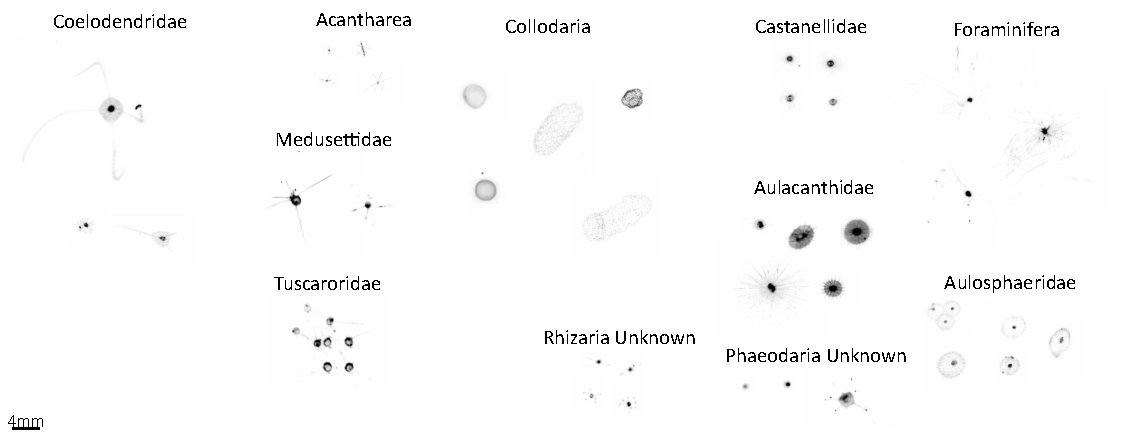
\includegraphics{images/01_taxa.pdf}

}

\caption{Example images of different Rhizaria taxa. 4mm scale bar shown
in lower right. All vignettes are same scale}

\end{figure}

The UVP5 samples at \textasciitilde15Hz rate as it descends the water
column and records the exact position of each particle larger than
600\(\mu m\). However, identified rhizaria ranged from a 934\(\mu m\)
Aulacanthidae cell to a Collodarian colony over 10mm in diameter. To
confirm that the UVP5 was sampling adequately across all size ranges, an
normalized biomass size spectrum (NBSS) slope was constructed to
identify a drop-off which would indicate poor-sampling at the small size
range (Barth and Stone, In press; Lombard et al., 2019). However, it was
evident from this analysis that all size ranges were adequately sampled
across the size range (Supplemental Figure 2) so no data were excluded.
The UVP5 reports the exact depth at which a particle is recorded,
however to estimate abundance, observations must be binned over fixed
depth intervals. Our deployments had variable descent depths and speeds
with more casts descending to 500m than 1000m and descents quicker
through the epipelagic than the mesopelagic (see Barth and Stone (2022)
for an extended discussion of UVP5 data processing). For the present
study, Rhizaria abundances were estimated in 25m vertical bins, which
offer a moderate sampling volume per bin (average 0.948\(m^3\) in the
epipelagic and 0.589\(m^3\) in the mesopelagic; Supplemental Table 1)
while still maintaining ecologically relevant widths. However,
concentrations in a 25m bin would need to be greater than 2.428 ind.
\(m^{-3}\) and 3.912 ind. \(m^{-3}\), in the epipelagic and mesopelagic
respectively, to fall below a 10\% non-detection risk (Barth and Stone,
In press; Benfield et al., 1996). Because we typically observed many
rhizaria taxa below these concentrations, we present the 25m binned data
to visualize broad-scale average distributions. For quantifying and
modelling Rhizaria abundances, we present integrated abundance
estimates, with each cast. Due to the variable descent depths of the
UVP, data are categorized as epipelagic (0-200m), upper mesopelagic
(200-500m), and lower mesopelagic (500-1000m). The average sampling
volume integrated through these regions were 7.59\(m^2\), 7.06\(m^2\),
and 11.77\(m^2\), with non-detection thresholds at 0.30 ind. \(m^{-2}\),
0.33 ind. \(m^{-2}\), and 0.20 ind. \(m^{-2}\) respectively. All UVP
data processing was done using the \texttt{EcotaxaTools} package in R
(Barth 2023).

\hypertarget{modelling-environmental-controls-of-rhizaria-abundance}{%
\subsection{Modelling environmental controls of Rhizaria
Abundance}\label{modelling-environmental-controls-of-rhizaria-abundance}}

Generalized Additive Models (GAMs) were used to assess the relationship
between integrated Rhizaria abundance and different environmental
factors. GAMs offer the ability to model non-linear and non-monotonic
relationships, which can be particularly useful in assessing ecological
relationships (Wood, 2017) and have been successfully applied to
Rhizaria ecology (Biard and Ohman, 2020). The \texttt{mgcv} package
(Wood, 2001) was used to construct models relating environmental
parameters to each taxonomic group's integrated abundance estimates from
each cast. To select the most parsimonious model for each analysis, a
backwards step-wise approach was taken. First, a full model was fit
using any term which may be ecologically relevant. Terms were fit using
maximum likelihood with a double penalty approach on unnecessary smooths
(Marra and Wood, 2011). The smoothness parameter was restricted (k = 6)
to prevent overfitting the models. At each iteration of the backwards
step-wise procedure, the model term with the lowest F score (least
statistically significant) was removed. This was repeated until all
model terms were statistically significant or the \(R^2_{adj}\) was
substantially reduced. Models were fit for each region; epipelagic,
upper mesopelagic, and lower mesopelagic. In cases where observations
were too sparse for a given taxonomic grouping, models were not run. All
code and full models are available in code, as well as intermediate data
products at \url{https://github.com/TheAlexBarth/RhizariaSeasonality}.

\hypertarget{results}{%
\section{Results}\label{results}}

\hypertarget{environmental-variability}{%
\subsubsection{Environmental
Variability}\label{environmental-variability}}

The BATS sampling region is southeast of Bermuda, situated in the
oligotrophic North Atlantic Subtropical Gyre. Due to the sampling
location, while the environmental conditions are generally low in
variation and oligotrophic, there is considerable influence from deep
winter-mixing and summer stratification as well as secondary influences
from mesoscale eddies which result in spatiotemporal heterogeniety
(Lomas et al., 2013; McGillicuddy et al., 1998). Variability in the
water column structure was visible during the study period (Figure 2).
This is best evidenced through the temperature profiles; In the late
summer and early fall there was a stratified water column with high
temperatures in the surface (\textless75m) (Figure 2A) and slightly
elevated salinity (Figure 2B). This warm, stratified period appeared
more intense during the few months sampled in 2019. In 2021, we observed
the stratified layer slowly dissipated into the winter months following
mixed layer entrainment. There was a consistent oxygen minimum zone
(OMZ) located at about 800m deep (Figure 2C). February 2021 saw a
notable downwelling event, likely due to a passing anti-cyclonic eddy
which impacted the local region during early 2021. During this phaes,
warmer, oxic water was significantly depressed deeper into the
mesopelagic. This process was reversed in the spring months (March,
April) primary due to the interaction of convective mixing and the
passing of a strong cyclonic eddy resulting in a deep cold mixed layer.
Primary production was highest during the spring mixing period,
evidenced both by in-situ fluorescence (Figure 2D) and productivity
incubation experiments (Figure 3A). Originating near the surface, the
productivity peak moved deeper throughout the spring and declined into
the summer (Figure 2D). However, there was a notable, yet smaller
productivity bump in the late summer and early fall (Figure 3A) which
occurred deeper in the epipelagic (Figure 2D). The particle
concentration (184\(\mu m\) - 450\(\mu m\)) was closely coupled to
chlorophyll-a patterns.

\begin{figure}

{\centering \includegraphics{images/02-environmental.pdf}

}

\caption{Environmental profiles across time-series of study period. Y
axis shows depth in meters. (A) Temperature. (B) Salinity. (C) Dissolved
Oxygen. (D) In-situ chlorophyll fluorescence. (E) Particle concenctrion
(184 - 450\(\mu m\)). (F) Bacteria Abundance. (G) Silica. (H) Nitrate}

\end{figure}

Overall, particle concentration was high near the surface during the
2021 spring bloom, then moved deeper throughout the water column
attenuating throughout the lower epipelagic (Figure 2E). Similarly,
heterotrophic bacteria abundance was closely linked to overall
productivity, althrough there was a more consistent moderate-abundance
layer near the top of the mesopelagic (\textasciitilde250m) (Figure 2F).
Concurrent with the secondary fall production peak, there was also
higher particle concentration and bacterial abundance in the later
summer and early fall. Interestingly, while primary productivity
estimates from July-August were not that different between 2019 and 2021
(Figure 3A), chlorophyll-a florescence, particle concentration, and
bacterial abundance were much higher in 2019's summer/fall (Figure
2D-F). Inorganic nutrients (\(Si\) and \(NO_3\)) were generally well
stratified, with low concentrations in the epipelagic and increasing
throughout the mesopelagic. However, both nutrients did vary vertically
in accordance with the 2021 February downwelling and spring mixing
period (Figure 2G-H). Additionally, in the late fall of 2021, \(Si\)
concentrations were slightly elevated in the mid-mesopelagic (Figure
2G).

\begin{figure}

{\centering 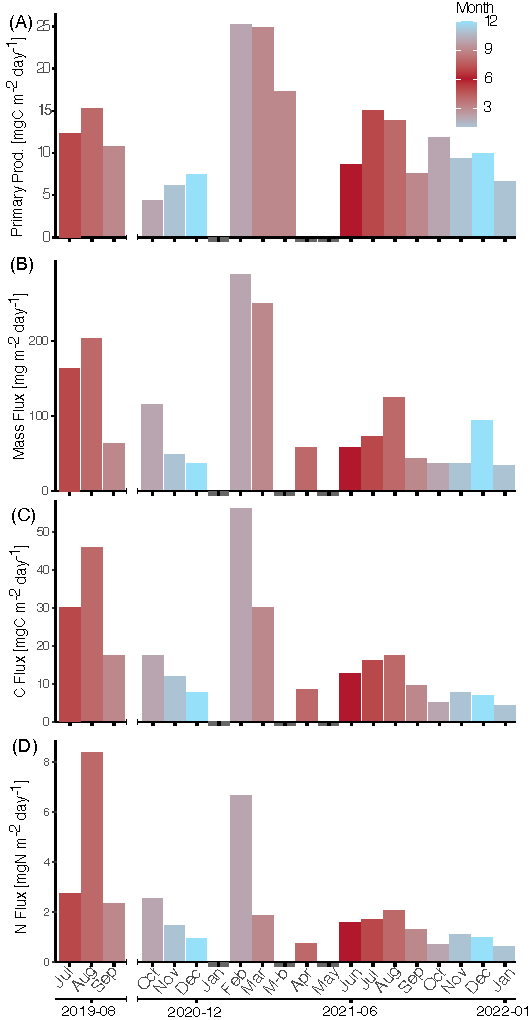
\includegraphics{images/03_prod-flux.pdf}

}

\caption{Primary productivity (A) and flux estimates from total mass
(B), carbon (C), and nitrogen (D). Values are from monthly cruises with
month displayed in corresponding colors. Absent data are shown by grey
bar.}

\end{figure}

Overall mass flux to the mesopelagic was highest during the 2021
February downwelling (Figure 3B). Generally, export was similarly high
during March, declining in April then increasing slightly throughout the
summer and early fall. While magnitude was slightly different, this
pattern was consistent with total mass, carbon and nitrogen fluxes
(Figure 3B-D). Higher mass, carbon and nitrogen flux also occurred in
the 2019 late summer - early fall period.

\hypertarget{rhizaria-abundance-and-distribution}{%
\subsubsection{Rhizaria abundance and
distribution}\label{rhizaria-abundance-and-distribution}}

Across all imaged mesozooplankton (\textgreater900\(\mu m\)), Rhizaria
comprised a considerable fraction of the total community. Considering
the total abundances of the observational period, Rhizaria comprised on
average, 42.6\% of all mesozooplankton abundance (Supplemental Figure
3). Copepods were the second most abundant, comprising 35.5\% and all
other living mesozooplankton were 22\%. The large contribution of
Rhizaria to the mesozooplankton community is most prominent in the
epipelagic, where they accounted for 47\% of all mesozooplankton. In the
mesopelagic rhizaria were a smaller (but still prominent fraction), at
38\% in the upper layers (200-500m) and 37\% in the deeper mesopelagic
(500-1000m).

\begin{figure}

{\centering 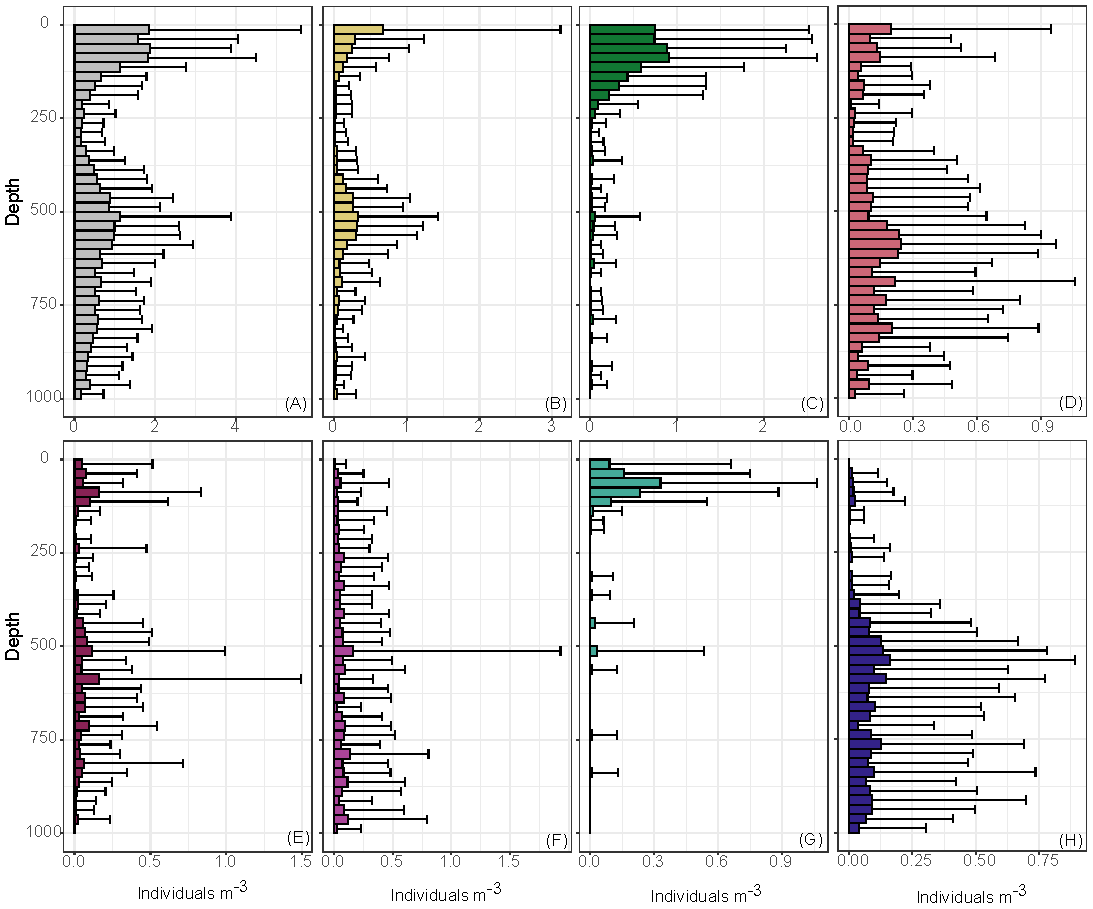
\includegraphics{images/04_vertical.pdf}

}

\caption{Average abundance of Rhizaria in 25m bins, across entire study
period. Shown are total Rhizaria (A), Acantharea (B), Collodaria (C),
Aulacanthidae (D), Foraminifera (E), Aulosphaeridae (F), Castanellidae
(G), Coelodendridae (H).}

\end{figure}

Total average Rhizaria abundance had a bimodal distribution with respect
to depth. Total abundance was highest just below the surface (0-100m),
with secondary, wider peak occurring in the mid mesopelagic (Figure 4A).
Variation in depth binned abundance was large, likely due to seasonal
variability but also increased from the detection-risk described in the
methods. The vertical distribution pattern and abundance varied
considerably across taxonomic groups. Radiolarias were some of the most
abundant taxa observed, particularly in the epipelagic (Figure 4, Figure
5B). This pattern was led by Collodaria, whose colonies were abundant in
the upper epipelagic and declined into the top of the mesopelagic
(Figure 4C). Acantharea displayed a bimodal distribution accounting for
a large portion of the total Rhizaria pattern (Figure 4B, Figure 5).
Foraminifera had a similar bimodal distribution, yet their overall
average densities were much lower and spread wider throughout the
mesopelagic (Figure 4E). Phaeodaria families exhibited a wide range of
vertical distribution patterns. The most abundant, Aulacanthidae, also
had a bimodal pattern but the density was highest in the lower
mesopelagic (Figure 4D). Aulosphaeridae had low average density and was
nearly homogeneously distributed throughout the water column, although
slightly lower in the epipelagic (Figure 4F). Castanellidae were the
only Phaeodaria who appeared to be effectively restricted to the photic
zone (Figure 4G). Alternatively, Coelodendridae primarily occurred in
the lower mesopelagic (Figure 4H). A few individuals from the families
Tuscaroridae and Medusettidae were also observed in the mesopelagic, yet
they were much rarer (data not shown).

\begin{figure}

{\centering 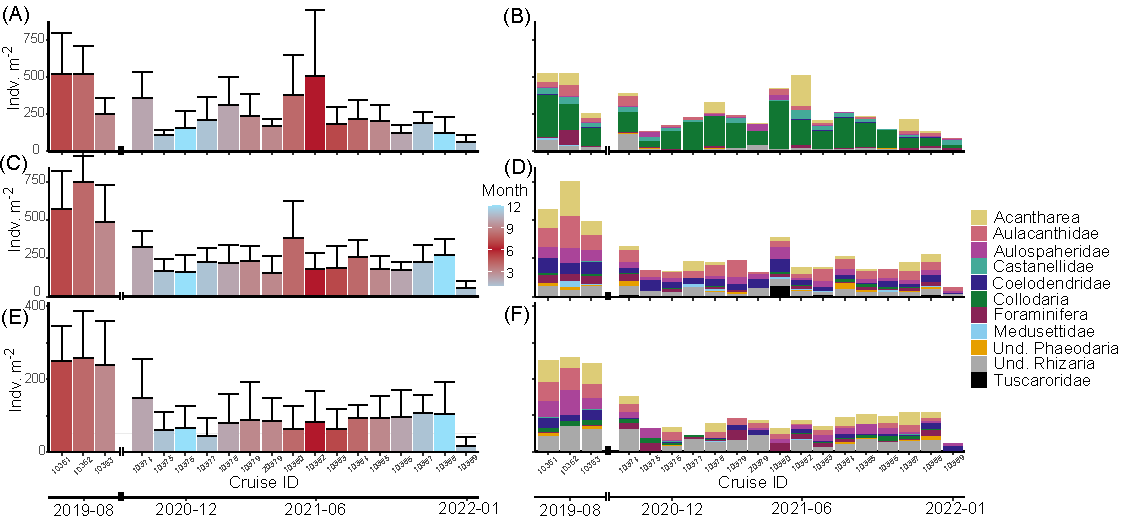
\includegraphics{images/05_seasonality.pdf}

}

\caption{Seasonality of Rhizaria integrated abundance for the epipelagic
(0-200m) (A-B), upper mesopelagic (200-500m) (C-D), lower mesopelagic
(500-1000m) (E-F). Left panels (A,C,E) display total integrated
abundance per monthly cruise colored by month. Right panels (B, D, F)
display community composition of each total abundance.}

\end{figure}

Between the monthly cruises, Rhizaria integrated abundance varied in the
epipelagic. Highest average abundance occurred in June 2021 and was
lowest during the winter months (Figure 5A). The 2019 later summer -
fall period also had much higher integrated abundance than similar
months in 2021. While the majority of integrated abundance in the
epipelagic was consistently attributable to Collodaria, Acanthrea
abundance occurred sporadically and could account for a large portion of
the total in some months (Figure 5B). The mesopelagic integrated
abundance was much more consistent across monthly cruises, although
average abundance was notably higher in 2019 (Figure 5C-F). The
community composition in the mesopelagic was more diverse, mostly
comprised of Phaeodarias. However, Acantharea and unidentified Rhizaria
also were common members of the community (Figure 5D, 5F).

\hypertarget{body-size-throughout-the-water-column.}{%
\subsubsection{Body size throughout the water
column.}\label{body-size-throughout-the-water-column.}}

Very few taxa had consistent distributions throughout the water column.
Only Acanthrea, Foraminifera, Aulacanthidae, and Aulosphaeridae were
consistently abundant in the epipelagic and mesopelagic. To investigate
if the populations or morphologies shifted throughout the water column,
we compared the sizes (Equivalent Spherical Diameters, ESD) between
mesopelagic and epipelagic groups for each taxa. All groups were
significantly different on average (Wilcox Rank Sum p-value
\textless0.001). Acantharea were smaller, on average in the mesopelagic
while all other taxa tended to be larger (Figure 6).

\begin{figure}

{\centering 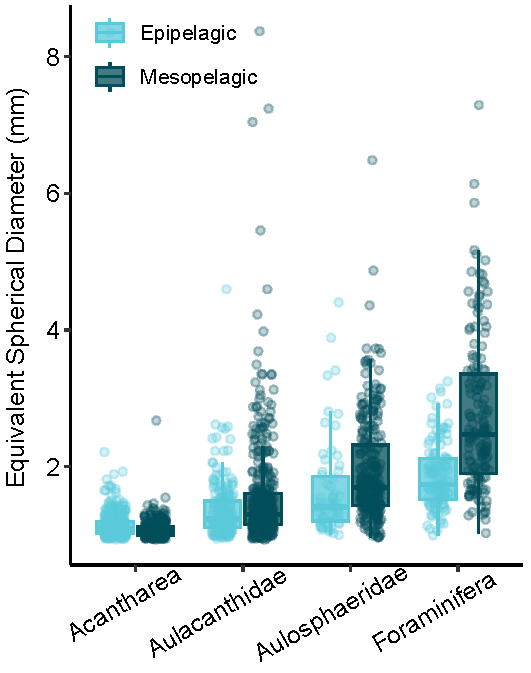
\includegraphics{images/09_size-comp.pdf}

}

\caption{Comparison of average sizes (ESD) amongst Rhizaria taxa which
occurred throughout the water column.}

\end{figure}

\hypertarget{environmental-drivers-of-rhizaria-abundance}{%
\subsubsection{Environmental Drivers of Rhizaria
Abundance}\label{environmental-drivers-of-rhizaria-abundance}}

For total Rhizaria integrated abundance the GAMs produced moderate fits
(\(R^2_{adj}\) = 0.406-0.603) (Table 1). In the epipelagic, there were
several significant predictor variables including inorganic nutrients
(\(NO_3\) and \(Si\)), water quality parameters (Salinity, DO), primary
production, and particle concentration (Table 1). However, the upper and
lower mesopelagic were exclusively explained by particle-related
variables (concentration and mass flux) (Table 1).

\begin{longtable}[]{@{}
  >{\raggedright\arraybackslash}p{(\columnwidth - 8\tabcolsep) * \real{0.4300}}
  >{\raggedright\arraybackslash}p{(\columnwidth - 8\tabcolsep) * \real{0.3400}}
  >{\raggedright\arraybackslash}p{(\columnwidth - 8\tabcolsep) * \real{0.0800}}
  >{\raggedright\arraybackslash}p{(\columnwidth - 8\tabcolsep) * \real{0.0800}}
  >{\raggedright\arraybackslash}p{(\columnwidth - 8\tabcolsep) * \real{0.0800}}@{}}
\caption{Generalized Additive Model results for integrated total
Rhizaria abundance in different regions of the water
column.}\tabularnewline
\toprule()
\begin{minipage}[b]{\linewidth}\raggedright
\textbf{Model}
\end{minipage} & \begin{minipage}[b]{\linewidth}\raggedright
Term
\end{minipage} & \begin{minipage}[b]{\linewidth}\raggedright
edf
\end{minipage} & \begin{minipage}[b]{\linewidth}\raggedright
F
\end{minipage} & \begin{minipage}[b]{\linewidth}\raggedright
p
\end{minipage} \\
\midrule()
\endfirsthead
\toprule()
\begin{minipage}[b]{\linewidth}\raggedright
\textbf{Model}
\end{minipage} & \begin{minipage}[b]{\linewidth}\raggedright
Term
\end{minipage} & \begin{minipage}[b]{\linewidth}\raggedright
edf
\end{minipage} & \begin{minipage}[b]{\linewidth}\raggedright
F
\end{minipage} & \begin{minipage}[b]{\linewidth}\raggedright
p
\end{minipage} \\
\midrule()
\endhead
\textbf{All Rhizaria Epipelagic} & Salinity & 2.0818 & 4.654 &
\textless0.001 \\
\(R^2_{adj}\)= 0.42 & DO & 0.8272 & 0.945 & 0.0136 \\
& Silica & 3.1206 & 15.75 & \textless0.001 \\
& NO3 & 2.9970 & 6.268 & \textless0.001 \\
& Primary Productivity & 1.8367 & 2.099 & \textless0.001 \\
& Particle Concentration & 0.9282 & 2.566 & \textless0.001 \\
\textbf{All Rhizaria Upper Mesopelagic} & Silica & 0.6847 & 0.431 &
0.073 \\
\(R^2_{adj}\)= 0.406 & Avg Mass Flux & 1.5426 & 0.923 & 0.045 \\
& Particle Concentration & 3.2957 & 20.89 & \textless0.001 \\
\textbf{All Rhizaria Lower Mesopelagic} & Avg Mass Flux & 1.6632 & 1.824
& 0.002 \\
\(R^2_{adj}\)= 0.603 & Particle Concentration & 0.7694 & 0.662 &
0.027 \\
\bottomrule()
\end{longtable}

GAMs for individual taxa were much less consistent in their fits (Table
2). This is likely in part due to the high number of non-observations
for certain taxa. Note that due to low abundances, GAMs were not
constructed for Tuscaroridae or Medusettidae. Furthermore no,
significant terms were found for a model with Aulosphaeridae in the
epipelagic nor Foraminifera in the mesopelagic.

\begin{figure}

{\centering 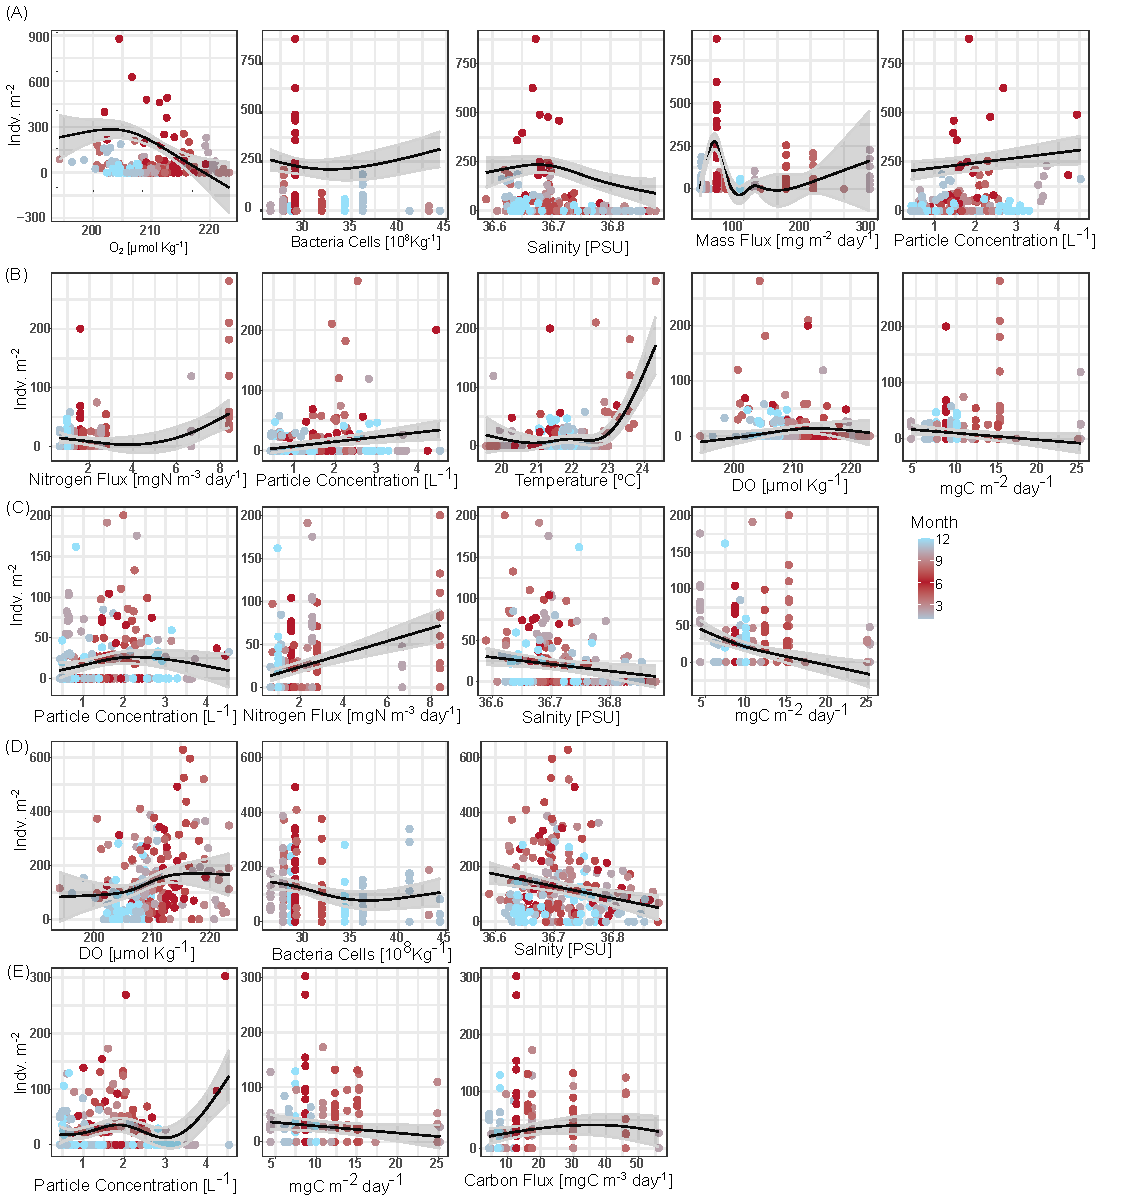
\includegraphics{images/06_epi-partials.pdf}

}

\caption{Partial effects of smooth terms in taxa-specific GAM models
from the epipelagic (0-200m). Effects are grouped by taxa; Acantharea
(A), Foraminifera (B), Aulacanthidae (C), Collodaria (D), Castanellidae
(E).}

\end{figure}

Epipelagic Acantharea were explained by several predictor variables and
had a good fit (\(R^2_{adj}\) = 0.53, Table 2). Most notable smooths
were mass flux and particle concentration, which had a weak positive
association (Figure 7A), with July 2021 as a clear outlier where
Acantharea abundances were high in the epipelagic despite lower fluxes
and particle concentrations (Figure 5). Foraminifera had a good fitting
GAM in the epipelagic (\(R^2_{adj}\) = 0.445). There were several
significant explanatory variables, although the clearest pattern was
observed of high temperatures associated with more Foraminifera
abundance (Table 2, Figure 7B). Epipelagic Aulacanthidae similarly had
several predictor variables which were significant, including both water
quality parameters and particle/flux predictors (Table 2).
Interestingly, Aulacanthidae had primary production as a significant
predictor, yet there was not a clear association (Figure 7C). There was
a fit for Collodaria in the epipelagic (\(R^2_{adj}\) = 0.16), although
there was a logit-like relationship where higher abundances tended to
occur during higher DO conditions in the surface waters (Figure 7D).
Castanellidae also had similarly poor fits in the epipelagic
(\(R^2_{adj}\) = 0.124) (Table 2, Figure 7E).

\begin{longtable}[]{@{}
  >{\raggedright\arraybackslash}p{(\columnwidth - 8\tabcolsep) * \real{0.4300}}
  >{\raggedright\arraybackslash}p{(\columnwidth - 8\tabcolsep) * \real{0.3400}}
  >{\raggedright\arraybackslash}p{(\columnwidth - 8\tabcolsep) * \real{0.0800}}
  >{\raggedright\arraybackslash}p{(\columnwidth - 8\tabcolsep) * \real{0.0800}}
  >{\raggedright\arraybackslash}p{(\columnwidth - 8\tabcolsep) * \real{0.0800}}@{}}
\caption{Taxa-specific generalized additive models for different regions
of the water column.}\tabularnewline
\toprule()
\begin{minipage}[b]{\linewidth}\raggedright
Model
\end{minipage} & \begin{minipage}[b]{\linewidth}\raggedright
Term
\end{minipage} & \begin{minipage}[b]{\linewidth}\raggedright
edf
\end{minipage} & \begin{minipage}[b]{\linewidth}\raggedright
F
\end{minipage} & \begin{minipage}[b]{\linewidth}\raggedright
p
\end{minipage} \\
\midrule()
\endfirsthead
\toprule()
\begin{minipage}[b]{\linewidth}\raggedright
Model
\end{minipage} & \begin{minipage}[b]{\linewidth}\raggedright
Term
\end{minipage} & \begin{minipage}[b]{\linewidth}\raggedright
edf
\end{minipage} & \begin{minipage}[b]{\linewidth}\raggedright
F
\end{minipage} & \begin{minipage}[b]{\linewidth}\raggedright
p
\end{minipage} \\
\midrule()
\endhead
\textbf{Acantharea Epipelagic} & Salinity & 2.264 & 4.113 &
\textless0.001 \\
R2adj=0.53 & O2 & 2.579 & 6.712 & \textless0.001 \\
& Avg Mass Flux & 4.810 & 22.81 & \textless0.001 \\
& Bacteria \#/L & 1.599 & 1.317 & 0.0117 \\
& Particle Concentration & 0.853 & 1.158 & 0.0087 \\
\textbf{Acantharea Upper Mesopelagic} & Avg C Flux & 1.296 & 0.621 &
0.0439 \\
R2adj=0.231 & Avg N Flux & 1.619 & 1.283 & 0.0026 \\
& Particle Concentration & 0.952 & 3.886 & \textless0.001 \\
\textbf{Acantharea Lower Mesopelagic} & Temperature & 2.076 & 4.155 &
\textless0.001 \\
R2adj=0.509 & Avg N Flux & 1.494 & 1.216 & 0.0113 \\
& Primary Productivity & 0.766 & 0.648 & 0.0253 \\
& Particle Concentration & 2.037 & 10.03 & \textless0.001 \\
\textbf{Aulacanthidae Epipelagic} & Salinity & 0.792 & 0.757 & 0.0241 \\
R2adj=0.251 & Avg N Flux & 0.869 & 1.324 & 0.0018 \\
& Primary Productivity & 2.312 & 7.704 & \textless0.001 \\
& Particle Concentration & 2.008 & 2.200 & 0.0017 \\
\textbf{Aulacanthidae Upper Mesopelagic} & Particle Concentration &
2.832 & 9.802 & \textless0.001 \\
R2adj = 0.158 & & & & \\
\textbf{Aulacanthidae Lower Mesopelagic} & Avg Mass Flux & 1.622 & 1.991
& 0.002 \\
R2adj=0.298 & Particle Concentration & 2.123 & 6.706 & \textless0.001 \\
\textbf{Aulosphaeridae Upper Mesopelagic} & Particle Concentration &
2.653 & 13.06 & \textless0.001 \\
R2adj=0.2 & & & & \\
\textbf{Aulosphaeridae Lower Mesopelagic} & Particle Concentration &
0.972 & 6.248 & \textless0.001 \\
R2adj=.147 & & & & \\
\textbf{Castanellidae Epipelagic} & Avg C Flux & 1.462 & 0.816 &
0.0421 \\
R2adj = 0.124 & Primary Productivity & 0.771 & 0.665 & 0.0247 \\
& Particle Concentration & 3.956 & 4.623 & \textless0.001 \\
\textbf{Coelodendridae Upper Mesopelagic} & Avg N Flux & 0.822 & 0.919 &
0.0183 \\
R2adj=.113 & Particle Concentration & 0.970 & 6.208 & \textless0.001 \\
\textbf{Coelodendridae Lower Mesopelagic} & Particle Concentration &
1.773 & 4.873 & \textless0.001 \\
R2adj=.133 & & & & \\
\textbf{Collodaria Epipelagic} & Salinity & 0.925 & 2.267 &
\textless0.001 \\
R2adj=0.16 & O2 & 2.015 & 2.217 & 0.002 \\
& Bacteria \#/L & 1.843 & 2.100 & 0.002 \\
\textbf{Foraminifera Epipelagic} & Temperature & 4.414 & 8.789 &
\textless0.001 \\
R2adj=0.445 & O2 & 1.603 & 1.287 & 0.0111 \\
& Avg N Flux & 2.512 & 3.396 & \textless0.001 \\
& Primary Productivity & 0.824 & 0.920 & 0.0153 \\
& Particle Concentration & 0.919 & 2.257 & \textless0.001 \\
\bottomrule()
\end{longtable}

\begin{figure}

{\centering 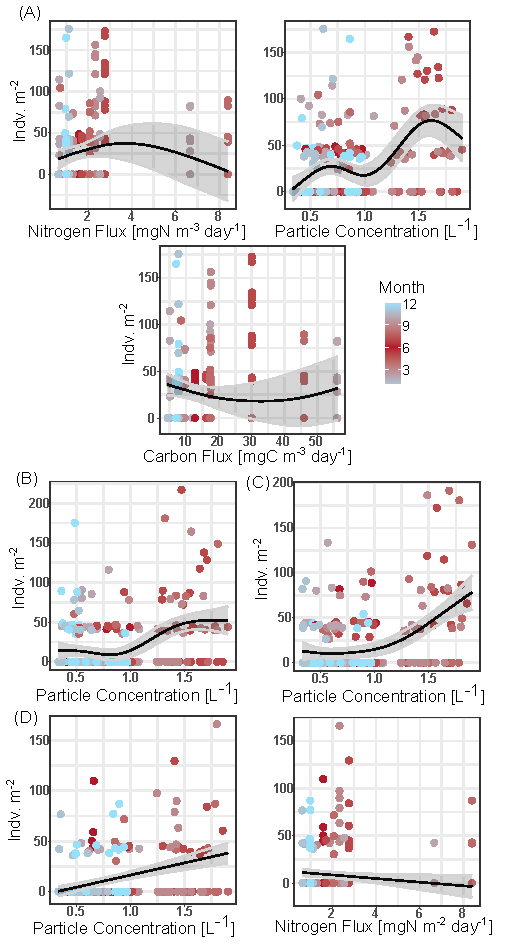
\includegraphics{images/07_upmeso-partial.pdf}

}

\caption{Partial effects of smooth terms in taxa-specific GAM models
from the upper mesopelagic (200-500m). Effects are grouped by taxa;
Acantharea (A), Aulacanthidae (B), Aulosphaeridae (C), Coelodendridae
(D).}

\end{figure}

In the upper mesopelagic (200-500m), abundances were generally low
(Figure 4) so GAMs were only constructed for Acantharea, Aulacanthidae,
Aulosphaeridae, and Coelodendridae (Table 2). All these models had
generally poor fits (\(R^2_{adj}\) \textless{} 0.25). Yet, for all upper
mesopelagic models, particle concentration was a significant explanatory
variable (Table 2, Figure 8). Carbon flux was significant for Acantharea
and nitrogen flux was significant for both Acantharea and Coelodendridae
(Table 2, Figure 8A,D). The lower mesopelagic also had generally poor
GAM fits for taxa specific models (\(R^2_{adj}\) \textless0.3), with the
exception of Acantharea (\(R^2_{adj}\) = 0.509). Acantharea in the lower
mesopelagic was most clearly positively associated with particle
concentration and nitrogen flux, as well as temperature to a slight
degree (Figure 9A). For all Phaeodarias with a significant model,
particle concentration was a main predictor variable (Table 2, Figure
9B-D). Aulacanthidae had the best fitting model of the Phaeodarias
(\(R^2_{adj}\) = 0.298), which also included mass flux as a
statistically significant smooth (Figure 9B).

\begin{figure}

{\centering 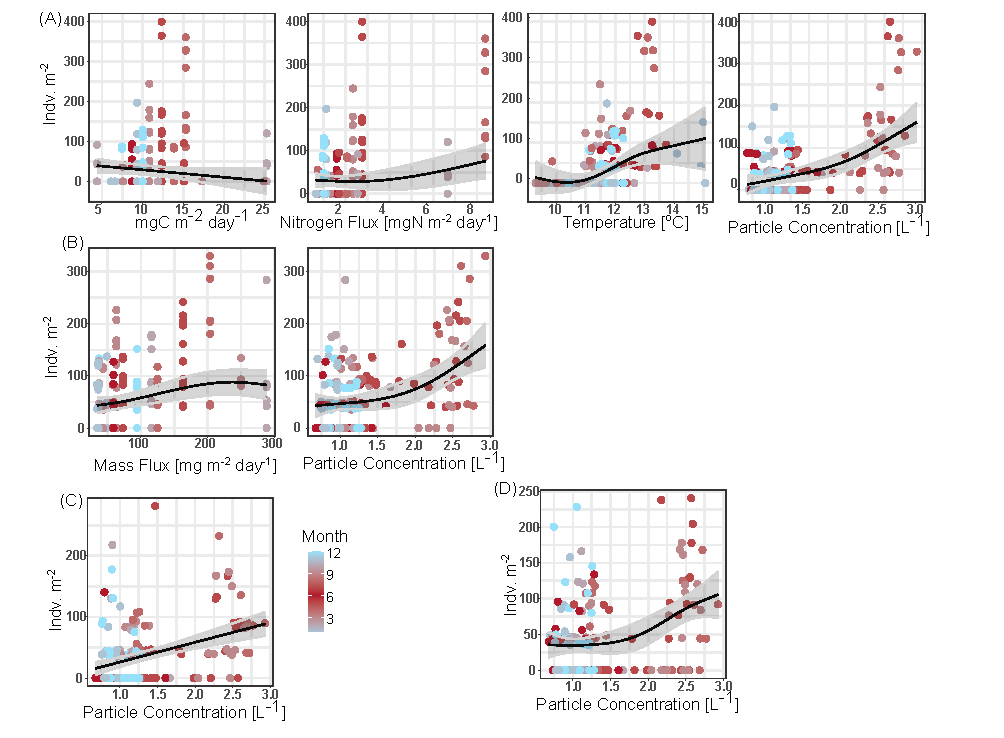
\includegraphics{images/08_lomeso-partials.pdf}

}

\caption{Partial effects of smooth terms in taxa-specific GAM models
from the lower mesopelagic (500-1000m). Effects are grouped by taxa;
Acantharea (A), Aulacanthidae (B), Aulosphaeridae (C), Coelodendridae
(D).}

\end{figure}

\hypertarget{discussion}{%
\section{Discussion}\label{discussion}}

\hypertarget{overall-rhizaria-abundance-and-patterns}{%
\subsubsection{Overall Rhizaria abundance and
patterns}\label{overall-rhizaria-abundance-and-patterns}}

In the epipelagic Rhizaria exhibited a notable seasonal pattern.
Rhizaria abundances were higher in the summer months and lower during
the winter. During a prior time period, Blanco-Bercial et al. (2022)
noted that there is considerable seasonality in the community
composition of all protists. Despite the seasonality of total Rhizaria
abundance, community composition was relatively consistent, with
Collodaria representing the bulk of the community. It should be noted
that the overall taxonomic resolution of the UVP5 is fairly low, so
there may be a switching of species within the broad groups identified
in this study which were not captured. Throughout the mesopelagic,
month-to-month variation in 2021 was relatively low. Again, this is
consistent with observations from metabarcoding of the whole protist
community in the same study region (Blanco-Bercial et al., 2022). This
finding is not surprising as the overall seasonal variation in
environmental conditions in this region were low.

Overall Rhizaria were the most commonly identified group of mesoplankton
throughout the study period. We do note that the UVP5 commonly captures
\emph{Trichodesmium} colonies, yet these were excluded in this
comparison as they are strictly autotrophs. It should be noted that
previous work has suggested that avoidance behavior with the UVP is
possible, at times likely, for visual and highly mobile zooplankton
(Barth and Stone, 2022). Thus, the percent contribution reported here
(42.7\%) of Rhizaria to the total mesozooplankton community may be
inflated due to under sampling of organisms such as Euphausiids and
Chaetognaths which have quick escape responses. Regardless, it is worth
noting that in the same region, with data collected in 2012 and 2013
using similar calculation methods, Biard et al. (2016) estimated
Rhizaria only contribute 15\% of the total mesozooplankton community in
the upper 500m. Likely, Rhizaria display considerable interannual
variability. In the present study, we noticed considerably higher
Rhizaria abundance throughout the water column in 2019 compared to 2021.
While this may have been driven by increased mass flux, more information
is needed to truly understand the magnitude by which Rhizaria can vary
interannually.

\hypertarget{relationship-to-environmental-parameters}{%
\subsubsection{Relationship to environmental
parameters}\label{relationship-to-environmental-parameters}}

In general, the fit of most GAMs were moderate to poor. One possible
reason for the poor fits may have been that for some taxa, conditions
were not variable enough to capture a range of conditions at which they
may exist. For instance, Collodaria were the most abundant taxa
observed, yet the fit of their GAM was particularly poor. In studies
which covered a wider range of parameters, Collodaria has been shown to
strongly vary with changes in parameters such as temperature,
chlorophyll-a, mixing, and water clarity (Biard et al., 2017; Biard and
Ohman, 2020). Alternatively, Acantharea had relatively good fitting
GAMs. These taxa also had some of the largest variation from month to
month on cruises. Thus, it may be that in the oligotrophic, the
relatively stable conditions can support certain taxa while others are
more sporadic. It should also be noted that due to the challenge of
adequately sampling enough volume to overcome low-detection issues, GAMs
were run on integrated data. However, variation with environmental
parameters throughout the water column are likely, just not captured in
the modelling aspect of this study. One consistent parameter which had
significant positive associations was particle concentration. This
observation is not surprising as most rhizaria likely to some extent
engage in flux feeding.

\hypertarget{vertical-structure-and-trophic-roles}{%
\subsubsection{Vertical Structure and Trophic
Roles}\label{vertical-structure-and-trophic-roles}}

In this study we present a clear pattern of vertical zonation between
different Rhizaria groups. Largely, the taxonomic composition and
vertical positioning were similar to Rhizaria zonation in the California
Current Ecosystem (Biard and Ohman, 2020). It should be noted however,
that the secondary abundance peak reported in the present study is
lower. This is likely due to the more oligotrophic nature of the study
region, were the euphotic zone penetrates deeper into the water column.
Most prevalent in the epipelagic were Collodaria. These mixotrophic
Radiolarians have long been reported to contribute to primary
productivity in the euphotic zone (Dennett et al., 2002; Michaels et
al., 1995). Collodaria are thought to be particularly successful
globally in oligotrophic regions due to their photosymbiotic
relationships (Biard et al., 2017, 2016). We observed the highest
abundance of Collodaria during June 2021, supporting the notion they can
thrive during the typically low-nutrient conditions of summer
stratification. However, Collodaria also increased during the spring
mixing period, suggesting that they can thrive during conditions which
may typically be thought to favor autotrophs. Furthermore, while
Collodaria were primarily absent from below 250m, there were a few
instances of deeper colonies being observed. Global investigations of
polycystine flux, suggest that deep-Collodaria in Oligotrophic regions
may be a consequence of isothermal submersion (Boltovskoy, 2017).
Alternatively, surface waters at BATS often mix into the mode water
during the seasonal mixing, so Collodaria in the deeper waters may be a
result of diapyncal mixing. Another effectively exclusively epipelagic
Rhizaria was the Phaeodaria family of Castanellidae. All Phaeodaria are
thought to be fully heterotrophic (Nakamura and Suzuki, 2015),
nonetheless a number of studies, including this one, report
Castanellidae to be typically found in the lower epipelagic (Biard et
al., 2018; Biard and Ohman, 2020; Zasko and Rusanov, 2005). It should be
considered that perhaps Castanellidae specializes in feeding on sinking
particles directly at the base of the epipelagic. Given it's smaller
size (Nakamura and Suzuki, 2015), Castanellidae does not need a large
diameter to efficiently flux feed at the typically particle rich region
of the lower epipelagic. Both Castanelldiae and Collodaria had poor
fitting GAMs. This is somewhat of a surprise for Collodaria who had
large abundance. However, given the consistency of their abundance, it
may be that this study did not capture a wide enough range of conditions
for describing Collodaria's preferred niche.

The mesopelagic generally was home to known heterotrophic organisms,
particularly for those which were constrained to exclusively occupy
deeper waters. This is consistent with Blanco-Bercial et al. (2022)'s
observation of an auto-/mixotroph to heterotroph gradient in the protist
community. The upper mesopelagic interestingly had relatively low total
abundance. This low-abundance region likely reflects the dynamics of
productivity and export throughout the water column. While productivity
and thus sinking particles for flux feeders are high in the euphotic
zone, much of this is attenuated throughout the epipelagic. So, while
the base of the epipelagic may provide a rich feeding environment for
Castanellidae, smaller protists, or heterotrophic bacteria (Figure 2F),
the region from 200-500m might be otherwise food poor. Perhaps it is
more advantageous for Rhizaria to situate deeper, in darker regions of
the twilight zone. Also it should be noted that Phaeodaria utilize
silica to build their opaline tests, and silica concentrations started
to increase around 500m (Figure 2G). Although \(Si\) was not a
significant smooth for any taxa-specific model, this lack of association
might be due to the overall lack of variation of \(Si\) between
integrated abundance of each cast. Aulosphaeridae was only found to have
significant relationships, although weak fits, to particle concentration
in the mesopelagic. In our study, while consistently observed, overall
abundances of Aulosphaeridae were very low. In the Pacific Ocean, on
California's Coast, much higher abundances of Aulosphaeridae have been
reported (Biard and Ohman, 2020; Zasko and Rusanov, 2005) and they have
massive potential to impact silica export (Biard et al., 2018).
Coelodendridae were also seemingly restricted to the deeper section of
the mesopelagic. This is interesting given that in the California
Current, (Biard and Ohman, 2020) found a bimodal distribution in
Coelodendridae. There are several morphotypes corresponding to different
taxa of Coelodendridae (Biard and Ohman, 2020; Nakamura and Suzuki,
2015). So it may be that only a few types of Coelodendridae were
observed in this study, while the epipelagic variety was not.
Alternatively, the lower epipelagic of the California Current may
provide adequate habitat for Coelodendridae, which is not available in
the oligotrophic Sargasso Sea.

A number of taxa were found to have a bimodal distribution, with
considerable populations in both the epipelagic and mesopelagic.
Aulacanthidae had a bimodal distribution, although abundances were
highest in the lower mesopelagic. Foraminifera also had a bimodal
distribution. Some lineages of Foraminifera are known to host
photosymbionts (Biard, 2022a; Kimoto, 2015), however they are also
efficient predators commonly seen throughout the mesopelagic (Caron and
Be, 1984; Gaskell et al., 2019). Thus it is not surprising to find their
presence in both locations of the water column. Foraminifera are also
known to vary their vertical distribution across their life cycle in
phase with lunar cycles (Biard, 2022a; Bijma et al., 1990; Gaskell et
al., 2019; Kimoto, 2015). However, the sampling scheme of the BATS
program does not capture this frequency and was not investigated in the
present study.

Acantharea also had a bimodal distribution, with much larger abundances
than Aulacanthidae or Foraminifera. Most prior studies of Acantharea
vertical distribution found them concentrated in near surface layers of
the water column Zasko and Rusanov (2005). This would support the
paradigm that large Acantharea abundances may be supported by their
mixotrophic abilities (Michaels et al., 1995; Suzuki and Not, 2015).
While the UVP5 images cannot distinguish between mixotrophic and
heterotrophic Acantharea, the GAMs constructed for Acantharea abundance
found positive associations with particle concentration and mass flux,
suggesting a higher reliance on heterotrophy. Recently Mars Brisbin et
al. (2020) described apparent predator behavior amongst near-surface
Acantharea. Thus it is likely that epipelagic Acantharea may commonly be
heterotrophic. Yet, it should be noted in the Sargasso Sea, both
heterotrophic and symbiotic lineages of Acantharea have been reported
(Blanco-Bercial et al., 2022). Additionally, Michaels (1988) noted that
the majority of Acantharea (by abundance) were smaller than
160\(\mu m\). While that estimate may be inflated due to inability to
capture larger cells, small Acantharea were not captured in the present
study. Thus, trophic strategy may shift based on sizes of Acantharea.

Decelle et al. (2013) proposed a hypothetical life cycle for
cyst-bearing (strictly heterotrophic) Acantharea. This hypothesized life
cycle suggests that epipelagic Acantharea are adult populations, which
form cysts that sink into the mesopelagic, then reproduce and rise.
Furthermore, given that horizontal transfer of symbionts between
generations of Acantharea is unlikely due to their spawning behavior,
the newly spawned mesopelagic Acantharea are not necessarily required to
rapidly return to the photic zone (Decelle et al., 2013, 2012). This
hypothesis predicts that Acanthareas in the mesopelagic would be smaller
(Decelle et al., 2013). Mars Brisbin et al. (2020) provided some support
for this hypothesis, with a significant decrease in Acantharea sizes
with depth. Although the authors also observed low abundances in the
mesopelagic and noted that the smaller sizes may be due to lower food
availability (Mars Brisbin et al., 2020). Since food is more scarce in
the mesopelagi, nutritional quality lower, yet flux feeders would likely
grow larger to increase their feeding range (Biard and Ohman, 2020). In
the data collecting in this study, Acanthareas in the mesopelagic were
significantly smaller than the epipelagic, despite the other bimodal
taxa (Foraminifera and Aulacanthidae) being significantly larger with
depth. This provides added support for the hypothesis that cyst-forming
Acantharea may utilize different sections of the water column throughout
their life cycle. However to further investigate this, more work is
needed with higher temporal and taxonomic resolution.

\hypertarget{conclusions-and-considerations}{%
\subsubsection{Conclusions and
Considerations}\label{conclusions-and-considerations}}

This study provides a detailed look at Rhizaria abundance over time
throughout the water column in a major oligotrophic gyre. We show that
their abundances are generally related to particle concentration and
flux, although lack of environmental variability may have reduced the
fit of our GAMs. Considering the potential role of Rhizaria in the
biological carbon pump, they may have a somewhat mixed role. In the
shallower regions, where smaller Rhizaria are abundant, they may be an
attenuating force on sinking particles (Stukel et al., 2019). It should
be noted that in our study, we focused on the ``small'' particle
concentration field (\textless450\(\mu m\)), and these particles are
generally slower sinking than large particles. However, once consumed
and repackaged by larger Rhizaria, they can sink quicker and contribute
more to overall flux (Michaels, 1988). Thus, Rhizaria may act as an
aggregation mechanism. However, this is largely speculation, to truly
test this, more work is needed measuring Rhizaria flux.

The vertical partitioning documented in this study do support the
hypothesis that mixotrophic rhizaria will occupy shallower waters while
deeper waters are dominated by heterotrophy. However the degree to which
mixotrophic Rhizaria in the euphotic zone rely on heterotrophy versus
symbiosis is uncertain. Collodaria were recorded as consistent and
dominant members of the near surface region. These organisms have the
potential to contribute considerably to the otherwise low productivity
of oligotrophic regions. However, their role in food webs is not well
understood. While this study represents a step-forward in our
understanding of Rhizaria ecology, continued research on Rhizaria is
much needed to better understand their ecology. Particularly extended
descriptive work to capture interannual patterns. Also work defining
biotic interactions, feeding rates, productivity, and life history are
all rich fields of interest in Rhizaria.

\hypertarget{references}{%
\section{References:}\label{references}}

\hypertarget{refs}{}
\begin{CSLReferences}{1}{0}
\leavevmode\vadjust pre{\hypertarget{ref-anderson2014}{}}%
Anderson, O.R., 2014. Living Together in the Plankton: A Survey of
Marine Protist Symbioses. Acta Protozoologica 53, 29--38.
\url{https://doi.org/10.4467/16890027AP.13.0019.1116}

\leavevmode\vadjust pre{\hypertarget{ref-anderson1976}{}}%
Anderson, O.R., Bé, A.W.H., 1976. A CYTOCHEMICAL FINE STRUCTURE STUDY OF
PHAGOTROPHY IN A PLANKTONIC FORAMINIFER, {\emph{HASTIGERINA PELAGICA}}
(d'ORBIGNY). The Biological Bulletin 151, 437--449.
\url{https://doi.org/10.2307/1540498}

\leavevmode\vadjust pre{\hypertarget{ref-aurahs2009}{}}%
Aurahs, R., Grimm, G.W., Hemleben, V., Hemleben, C., Kucera, M., 2009.
Geographical distribution of cryptic genetic types in the planktonic
foraminifer Globigerinoides ruber. Molecular Ecology 18, 1692--1706.
\url{https://doi.org/10.1111/j.1365-294X.2009.04136.x}

\leavevmode\vadjust pre{\hypertarget{ref-barth-inpress}{}}%
Barth, A., Stone, J., In press. Understanding the picture: The promis
and challenges of in-situ imagery data in the study of plankton ecology.
Journal of Plankton Research: Horizons.

\leavevmode\vadjust pre{\hypertarget{ref-barth2022}{}}%
Barth, A., Stone, J., 2022.
\href{https://www.frontiersin.org/articles/10.3389/fmars.2022.898057}{Comparison
of an in situ imaging device and net-based method to study
mesozooplankton communities in an oligotrophic system}. Frontiers in
Marine Science 9.

\leavevmode\vadjust pre{\hypertarget{ref-benfield1996}{}}%
Benfield, M.C., Davis, C.S., Wiebe, P.H., Gallager, S.M., Gregory Lough,
R., Copley, N.J., 1996. Video Plankton Recorder estimates of copepod,
pteropod and larvacean distributions from a stratified region of Georges
Bank with comparative measurements from a MOCNESS sampler. Deep Sea
Research Part II: Topical Studies in Oceanography 43, 1925--1945.
\url{https://doi.org/10.1016/S0967-0645(96)00044-6}

\leavevmode\vadjust pre{\hypertarget{ref-biard2022}{}}%
Biard, T., 2022a. Rhizaria. Encyclopeida of Life Sciences, pp. 1--11.
\url{https://doi.org/10.1002/9780470015902.a0029469}

\leavevmode\vadjust pre{\hypertarget{ref-biard2022b}{}}%
Biard, T., 2022b. Diversity and ecology of Radiolaria in modern oceans.
Environmental Microbiology 24, 2179--2200.
\url{https://doi.org/10.1111/1462-2920.16004}

\leavevmode\vadjust pre{\hypertarget{ref-biard2017}{}}%
Biard, T., Bigeard, E., Audic, S., Poulain, J., Gutierrez-Rodriguez, A.,
Pesant, S., Stemmann, L., Not, F., 2017. Biogeography and diversity of
Collodaria (Radiolaria) in the global ocean. The ISME Journal 11,
1331--1344. \url{https://doi.org/10.1038/ismej.2017.12}

\leavevmode\vadjust pre{\hypertarget{ref-biard2018}{}}%
Biard, T., Krause, J.W., Stukel, M.R., Ohman, M.D., 2018. The
Significance of Giant Phaeodarians (Rhizaria) to Biogenic Silica Export
in the California Current Ecosystem. Global Biogeochemical Cycles 32,
987--1004. \url{https://doi.org/10.1029/2018GB005877}

\leavevmode\vadjust pre{\hypertarget{ref-biard2020}{}}%
Biard, T., Ohman, M.D., 2020. Vertical niche definition of test-bearing
protists (Rhizaria) into the twilight zone revealed by in situ imaging.
Limnology and Oceanography 65, 2583--2602.
\url{https://doi.org/10.1002/lno.11472}

\leavevmode\vadjust pre{\hypertarget{ref-biard2015}{}}%
Biard, T., Pillet, L., Decelle, J., Poirier, C., Suzuki, N., Not, F.,
2015. Towards an integrative morpho-molecular classification of the
collodaria (polycystinea, radiolaria). Protist 166, 374--388.
\url{https://doi.org/10.1016/j.protis.2015.05.002}

\leavevmode\vadjust pre{\hypertarget{ref-biard2016}{}}%
Biard, T., Stemmann, L., Picheral, M., Mayot, N., Vandromme, P., Hauss,
H., Gorsky, G., Guidi, L., Kiko, R., Not, F., 2016. In situ imaging
reveals the biomass of giant protists in the global ocean. Nature 532,
504--507. \url{https://doi.org/10.1038/nature17652}

\leavevmode\vadjust pre{\hypertarget{ref-bijma1990}{}}%
Bijma, J., Erez, J., Hemleben, C., 1990.
\href{https://epic.awi.de/id/eprint/6096/1/Bij1990a.pdf}{Lunar and
semi-luan reproductive cycles in some spinose planktonic foraminifers}.
Journal of Foraminiferal Research 20, 117--127.

\leavevmode\vadjust pre{\hypertarget{ref-blanco-bercial2022}{}}%
Blanco-Bercial, L., Parsons, R., Bolaños, L.M., Johnson, R., Giovannoni,
S.J., Curry, R., 2022.
\href{https://www.frontiersin.org/articles/10.3389/fmars.2022.897140}{The
protist community traces seasonality and mesoscale hydrographic features
in the oligotrophic sargasso sea}. Frontiers in Marine Science 9.

\leavevmode\vadjust pre{\hypertarget{ref-boltovskoy2017}{}}%
Boltovskoy, D., 2017. Vertical distribution patterns of radiolaria
polycystina (protista) in the world ocean: Living ranges, isothermal
submersion and settling shells. Journal of Plankton Research 39,
330--349. \url{https://doi.org/10.1093/plankt/fbx003}

\leavevmode\vadjust pre{\hypertarget{ref-boltovskoy1993}{}}%
Boltovskoy, D., Alder, V.A., Abelmann, A., 1993. Annual flux of
radiolaria and other shelled plankters in the eastern equatorial
atlantic at 853 m: seasonal variations and polycystine species-specific
responses. Deep Sea Research Part I: Oceanographic Research Papers 40,
1863--1895. \url{https://doi.org/10.1016/0967-0637(93)90036-3}

\leavevmode\vadjust pre{\hypertarget{ref-caron2016}{}}%
Caron, D.A., 2016.
\href{https://www.nature.com/articles/nature17892}{The rise of rhizaria
\textbar{} nature}. Nature 532, 444--445.

\leavevmode\vadjust pre{\hypertarget{ref-caron1984}{}}%
Caron, D.A., Be, A.W.H., 1984. PREDICTED AND OBSERVED FEEDING RATES OF
THE SPINOSE PLANKTONIC FORAMINIFER. BULLETIN OF MARINE SCIENCE 35.

\leavevmode\vadjust pre{\hypertarget{ref-caron1995}{}}%
Caron, D.A., Michaels, A.F., Swanberg, N.R., Howse, F.A., 1995. Primary
productivity by symbiont-bearing planktonic sarcodines (acantharia,
radiolaria, foraminifera) in surface waters near bermuda. Journal of
Plankton Research 17, 103--129.
\url{https://doi.org/10.1093/plankt/17.1.103}

\leavevmode\vadjust pre{\hypertarget{ref-cavalier-smith2018}{}}%
Cavalier-Smith, T., Chao, E.E., Lewis, R., 2018. Multigene phylogeny and
cell evolution of chromist infrakingdom Rhizaria: contrasting cell
organisation~of sister~phyla Cercozoa and Retaria. Protoplasma 255,
1517--1574. \url{https://doi.org/10.1007/s00709-018-1241-1}

\leavevmode\vadjust pre{\hypertarget{ref-cohen2023}{}}%
Cohen, N.R., Krinos, A.I., Kell, R.M., Chmiel, R.J., Moran, D.M.,
McIlvin, M.R., Lopez, P.Z., Barth, A., Stone, J., Alanis, B.A., Chan,
E.W., Breier, J.A., Jakuba, M.V., Johnson, R., Alexander, H., Saito,
M.A., 2023. Microeukaryote metabolism across the western North Atlantic
Ocean revealed through autonomous underwater profiling.
\url{https://doi.org/10.1101/2023.11.20.567900}

\leavevmode\vadjust pre{\hypertarget{ref-decelle2015}{}}%
Decelle, J., Colin, S., Foster, R.A., 2015. Photosymbiosis in Marine
Planktonic Protists, in: Ohtsuka, S., Suzaki, T., Horiguchi, T., Suzuki,
N., Not, F. (Eds.),. Springer Japan, Tokyo, pp. 465--500.
\url{https://doi.org/10.1007/978-4-431-55130-0_19}

\leavevmode\vadjust pre{\hypertarget{ref-decelle2013}{}}%
Decelle, J., Martin, P., Paborstava, K., Pond, D.W., Tarling, G., Mahé,
F., De Vargas, C., Lampitt, R., Not, F., 2013. Diversity, Ecology and
Biogeochemistry of Cyst-Forming Acantharia (Radiolaria) in the Oceans.
PLoS ONE 8, e53598. \url{https://doi.org/10.1371/journal.pone.0053598}

\leavevmode\vadjust pre{\hypertarget{ref-decelle2012}{}}%
Decelle, J., Siano, R., Probert, I., Poirier, C., Not, F., 2012.
Multiple microalgal partners in symbiosis with the acantharian
Acanthochiasma sp. (Radiolaria). Symbiosis 58, 233--244.
\url{https://doi.org/10.1007/s13199-012-0195-x}

\leavevmode\vadjust pre{\hypertarget{ref-dennett2002}{}}%
Dennett, M.R., Caron, D.A., Michaels, A.F., Gallager, S.M., Davis, C.S.,
2002. Video plankton recorder reveals high abundances of colonial
radiolaria in surface waters of the central north pacific. Journal of
Plankton Research 24, 797--805.
\url{https://doi.org/10.1093/plankt/24.8.797}

\leavevmode\vadjust pre{\hypertarget{ref-drago2022}{}}%
Drago, L., Panaïotis, T., Irisson, J.-O., Babin, M., Biard, T.,
Carlotti, F., Coppola, L., Guidi, L., Hauss, H., Karp-Boss, L., Lombard,
F., Mcdonnell, A.M.P., Picheral, M., Rogge, A., Waite, A.M., Stemmann,
L., Kiko, R., 2022. Global Distribution of Zooplankton Biomass Estimated
by In Situ Imaging and Machine Learning. Frontiers in Marine Science 9.
\url{https://doi.org/10.3389/fmars.2022.894372}

\leavevmode\vadjust pre{\hypertarget{ref-gaskell2019}{}}%
Gaskell, D.E., Ohman, M.D., Hull, P.M., 2019. Zooglider-based
measurements of planktonic foraminifera in the california current
system. Journal of Foraminiferal Research 49, 390--404.
\url{https://doi.org/10.2113/gsjfr.49.4.390}

\leavevmode\vadjust pre{\hypertarget{ref-guidi2016}{}}%
Guidi, L., Chaffron, S., Bittner, L., Eveillard, D., Larhlimi, A., Roux,
S., Darzi, Y., Audic, S., Berline, L., Brum, J.R., Coelho, L.P.,
Espinoza, J.C.I., Malviya, S., Sunagawa, S., Dimier, C., Kandels-Lewis,
S., Picheral, M., Poulain, J., Searson, S., Stemmann, L., Not, F.,
Hingamp, P., Speich, S., Follows, M., Karp-Boss, L., Boss, E., Ogata,
H., Pesant, S., Weissenbach, J., Wincker, P., Acinas, S.G., Bork, P.,
Vargas, C. de, Iudicone, D., Sullivan, M.B., Raes, J., Karsenti, E.,
Bowler, C., Gorsky, G., 2016. Plankton networks driving carbon export in
the oligotrophic ocean. Nature 532, 465--470.
\url{https://doi.org/10.1038/nature16942}

\leavevmode\vadjust pre{\hypertarget{ref-gutierrez-rodriguez2019}{}}%
Gutierrez-Rodriguez, A., Stukel, M.R., Lopes dos Santos, A., Biard, T.,
Scharek, R., Vaulot, D., Landry, M.R., Not, F., 2019. High contribution
of Rhizaria (Radiolaria) to vertical export in the California Current
Ecosystem revealed by DNA metabarcoding. The ISME Journal 13, 964--976.
\url{https://doi.org/10.1038/s41396-018-0322-7}

\leavevmode\vadjust pre{\hypertarget{ref-gutiuxe9rrez-rodruxedguez2022}{}}%
Gutiérrez-Rodríguez, A., Lopes dos Santos, A., Safi, K., Probert, I.,
Not, F., Fernández, D., Gourvil, P., Bilewitch, J., Hulston, D.,
Pinkerton, M., Nodder, S.D., 2022. Planktonic protist diversity across
contrasting subtropical and subantarctic waters of the southwest
pacific. Progress in Oceanography 206, 102809.
\url{https://doi.org/10.1016/j.pocean.2022.102809}

\leavevmode\vadjust pre{\hypertarget{ref-haekel1887}{}}%
Haekel, E., 1887.
\href{https://www.gutenberg.org/cache/epub/44527/pg44527-images.html}{Report
on the radiolaria collected by h.m.s. Challenger during the years
1873-1876, plates, by ernst haeckel}.

\leavevmode\vadjust pre{\hypertarget{ref-hull2011}{}}%
Hull, P.M., Osborn, K.J., Norris, R.D., Robison, B.H., 2011. Seasonality
and depth distribution of a mesopelagic foraminifer, Hastigerinella
digitata, in Monterey Bay, California. Limnology and Oceanography 56,
562--576. \url{https://doi.org/10.4319/lo.2011.56.2.0562}

\leavevmode\vadjust pre{\hypertarget{ref-ikenoue2019}{}}%
Ikenoue, T., Kimoto, K., Okazaki, Y., Sato, M., Honda, M.C., Takahashi,
K., Harada, N., Fujiki, T., 2019. Phaeodaria: An Important Carrier of
Particulate Organic Carbon in the Mesopelagic Twilight Zone of the North
Pacific Ocean. Global Biogeochemical Cycles 33, 1146--1160.
\url{https://doi.org/10.1029/2019GB006258}

\leavevmode\vadjust pre{\hypertarget{ref-kimoto2015}{}}%
Kimoto, K., 2015. Planktic foraminifera. pp. 129--178.
\url{https://doi.org/10.1007/978-4-431-55130-0_7}

\leavevmode\vadjust pre{\hypertarget{ref-knap1997}{}}%
Knap, A.H., Michaels, A.F., Steinberg, D.K., Bahr, F., Bates, N.R.,
Bell, S., Countway, P., Close, A.R., Doyle, A.P., Dow, R.L., Howse,
F.A., Gundersen, K., Johnson, R.J., Kelly, R., Little, R., Orcutt, K.,
Parsons, R., Rathburn, C., Sanderson, M., Stone, S., 1997.
\href{https://eprints.soton.ac.uk/361194/}{BATS methods manual, version
4}.

\leavevmode\vadjust pre{\hypertarget{ref-laget2024}{}}%
Laget, M., Drago, L., Panaïotis, T., Kiko, R., Stemmann, L., Rogge, A.,
Llopis-Monferrer, N., Leynaert, A., Irisson, J.-O., Biard, T., 2024.
Global census of the significance of giant mesopelagic protists to the
marine carbon and silicon cycles. Nature Communications 15, 3341.
\url{https://doi.org/10.1038/s41467-024-47651-4}

\leavevmode\vadjust pre{\hypertarget{ref-lampitt2009}{}}%
Lampitt, R.S., Salter, I., Johns, D., 2009. Radiolaria: Major exporters
of organic carbon to the deep ocean. Global Biogeochemical Cycles 23.
\url{https://doi.org/10.1029/2008GB003221}

\leavevmode\vadjust pre{\hypertarget{ref-lee2006}{}}%
Lee, J.J., 2006.
\href{https://dalspace.library.dal.ca/bitstream/handle/10222/78255/VOLUME\%2042-NUMBER\%202-2006-PAGE\%2063.pdf?sequence=1}{Algal
symbiosis in larger foraminifera}. Symbiosis 42, 63--75.

\leavevmode\vadjust pre{\hypertarget{ref-llopismonferrer2022}{}}%
Llopis Monferrer, N., Biard, T., Sandin, M.M., Lombard, F., Picheral,
M., Elineau, A., Guidi, L., Leynaert, A., Tréguer, P.J., Not, F., 2022.
\href{https://www.frontiersin.org/articles/10.3389/fmars.2022.895995}{Siliceous
rhizaria abundances and diversity in the mediterranean sea assessed by
combined imaging and metabarcoding approaches}. Frontiers in Marine
Science 9.

\leavevmode\vadjust pre{\hypertarget{ref-llopismonferrer2021}{}}%
Llopis Monferrer, N., Leynaert, A., Tréguer, P., Gutiérrez-Rodríguez,
A., Moriceau, B., Gallinari, M., Latasa, M., L'Helguen, S., Maguer,
J.-F., Safi, K., Pinkerton, M.H., Not, F., 2021. Role of small Rhizaria
and diatoms in the pelagic silica production of the Southern Ocean.
Limnology and Oceanography 66, 2187--2202.
\url{https://doi.org/10.1002/lno.11743}

\leavevmode\vadjust pre{\hypertarget{ref-lomas2013}{}}%
Lomas, M.W., Bates, N.R., Johnson, R.J., Knap, A.H., Steinberg, D.K.,
Carlson, C.A., 2013. Two decades and counting: 24-years of sustained
open ocean biogeochemical measurements in the Sargasso Sea. Deep Sea
Research Part II: Topical Studies in Oceanography 93, 16--32.
\url{https://doi.org/10.1016/j.dsr2.2013.01.008}

\leavevmode\vadjust pre{\hypertarget{ref-lombard2019}{}}%
Lombard, F., Boss, E., Waite, A.M., Vogt, M., Uitz, J., Stemmann, L.,
Sosik, H.M., Schulz, J., Romagnan, J.-B., Picheral, M., Pearlman, J.,
Ohman, M.D., Niehoff, B., Möller, K.O., Miloslavich, P., Lara-Lpez, A.,
Kudela, R., Lopes, R.M., Kiko, R., Karp-Boss, L., Jaffe, J.S., Iversen,
M.H., Irisson, J.-O., Fennel, K., Hauss, H., Guidi, L., Gorsky, G.,
Giering, S.L.C., Gaube, P., Gallager, S., Dubelaar, G., Cowen, R.K.,
Carlotti, F., Briseño-Avena, C., Berline, L., Benoit-Bird, K., Bax, N.,
Batten, S., Ayata, S.D., Artigas, L.F., Appeltans, W., 2019.
\href{https://www.frontiersin.org/articles/10.3389/fmars.2019.00196}{Globally
consistent quantitative observations of planktonic ecosystems}.
Frontiers in Marine Science 6.

\leavevmode\vadjust pre{\hypertarget{ref-marra2011}{}}%
Marra, G., Wood, S.N., 2011. Practical variable selection for
generalized additive models. Computational Statistics \& Data Analysis
55, 2372--2387. \url{https://doi.org/10.1016/j.csda.2011.02.004}

\leavevmode\vadjust pre{\hypertarget{ref-marsbrisbin2020}{}}%
Mars Brisbin, M., Brunner, O.D., Grossmann, M.M., Mitarai, S., 2020.
Paired high-throughput, in situ imaging and high-throughput sequencing
illuminate acantharian abundance and vertical distribution. Limnology
and Oceanography 65, 2953--2965. \url{https://doi.org/10.1002/lno.11567}

\leavevmode\vadjust pre{\hypertarget{ref-mcgillicuddy1998}{}}%
McGillicuddy, D.J., Robinson, A.R., Siegel, D.A., Jannasch, H.W.,
Johnson, R., Dickey, T.D., McNeil, J., Michaels, A.F., Knap, A.H., 1998.
Influence of mesoscale eddies on new production in the Sargasso Sea.
Nature 394, 263--266. \url{https://doi.org/10.1038/28367}

\leavevmode\vadjust pre{\hypertarget{ref-michaels1988}{}}%
Michaels, A.F., 1988. Vertical distribution and abundance of Acantharia
and their symbionts. Marine Biology 97, 559--569.
\url{https://doi.org/10.1007/BF00391052}

\leavevmode\vadjust pre{\hypertarget{ref-michaels1995}{}}%
Michaels, A.F., Caron, D.A., Swanberg, N.R., Howse, F.A., Michaels,
C.M., 1995. Planktonic sarcodines (Acantharia, Radiolaria, Foraminifera)
in surface waters near Bermuda: abundance, biomass and vertical flux.
Journal of Plankton Research 17, 131--163.
\url{https://doi.org/10.1093/plankt/17.1.131}

\leavevmode\vadjust pre{\hypertarget{ref-michaels1996}{}}%
Michaels, A.F., Knap, A.H., 1996. Overview of the U.S. JGOFS Bermuda
Atlantic Time-series Study and the Hydrostation S program. Deep Sea
Research Part II: Topical Studies in Oceanography 43, 157--198.
\url{https://doi.org/10.1016/0967-0645(96)00004-5}

\leavevmode\vadjust pre{\hypertarget{ref-nakamura2023}{}}%
Nakamura, Y., Itagaki, H., Tuji, A., Shimode, S., Yamaguchi, A., Hidaka,
K., Ogiso-Tanaka, E., 2023. DNA metabarcoding focused on
difficult-to-culture protists: An effective approach to clarify
biological interactions. Environmental Microbiology 25, 3630--3638.
\url{https://doi.org/10.1111/1462-2920.16524}

\leavevmode\vadjust pre{\hypertarget{ref-nakamura2015}{}}%
Nakamura, Y., Suzuki, N., 2015.
\href{https://link.springer.com/chapter/10.1007/978-4-431-55130-0_9}{Phaeodaria:
Diverse marine cercozoans of world-wide distribution}. Springer, pp.
223--249.

\leavevmode\vadjust pre{\hypertarget{ref-ohman2019a}{}}%
Ohman, M.D., 2019. A sea of tentacles: optically discernible traits
resolved from planktonic organisms in situ. ICES Journal of Marine
Science 76, 1959--1972. \url{https://doi.org/10.1093/icesjms/fsz184}

\leavevmode\vadjust pre{\hypertarget{ref-panauxefotis2023}{}}%
Panaïotis, T., Babin, M., Biard, T., Carlotti, F., Coppola, L., Guidi,
L., Hauss, H., Karp-Boss, L., Kiko, R., Lombard, F., McDonnell, A.M.P.,
Picheral, M., Rogge, A., Waite, A.M., Stemmann, L., Irisson, J.-O.,
2023. Three major mesoplanktonic communities resolved by in situ imaging
in the upper 500 m of the global ocean. Global Ecology and Biogeography
32, 1991--2005. \url{https://doi.org/10.1111/geb.13741}

\leavevmode\vadjust pre{\hypertarget{ref-picheral}{}}%
Picheral, M., Colin, S.P., Irisson, J.-O., n.d.
\href{https://ecotaxa.obs-vlfr.fr/}{Ecotaxa}.

\leavevmode\vadjust pre{\hypertarget{ref-picheral2010}{}}%
Picheral, M., Guidi, L., Stemmann, L., Karl, D.M., Iddaoud, G., Gorsky,
G., 2010. The Underwater Vision Profiler 5: An advanced instrument for
high spatial resolution studies of particle size spectra and
zooplankton. Limnology and Oceanography: Methods 8, 462--473.
\url{https://doi.org/10.4319/lom.2010.8.462}

\leavevmode\vadjust pre{\hypertarget{ref-sogawa2022}{}}%
Sogawa, S., Nakamura, Y., Nagai, S., Nishi, N., Hidaka, K., Shimizu, Y.,
Setou, T., 2022. DNA metabarcoding reveals vertical variation and hidden
diversity of alveolata and rhizaria communities in the western north
pacific. Deep Sea Research Part I: Oceanographic Research Papers 183,
103765. \url{https://doi.org/10.1016/j.dsr.2022.103765}

\leavevmode\vadjust pre{\hypertarget{ref-stukel2018}{}}%
Stukel, M.R., Biard, T., Krause, J., Ohman, M.D., 2018. Large Phaeodaria
in the twilight zone: Their role in the carbon cycle. Limnology and
Oceanography 63, 2579--2594. \url{https://doi.org/10.1002/lno.10961}

\leavevmode\vadjust pre{\hypertarget{ref-stukel2019}{}}%
Stukel, M.R., Ohman, M.D., Kelly, T.B., Biard, T., 2019.
\href{https://www.frontiersin.org/articles/10.3389/fmars.2019.00397}{The
roles of suspension-feeding and flux-feeding zooplankton as gatekeepers
of particle flux into the mesopelagic ocean in the northeast pacific}.
Frontiers in Marine Science 6.

\leavevmode\vadjust pre{\hypertarget{ref-suzuki2015}{}}%
Suzuki, N., Not, F., 2015.
\href{https://link.springer.com/chapter/10.1007/978-4-431-55130-0_8}{Biology
and ecology of radiolaria}. Springer, pp. 179--222.

\leavevmode\vadjust pre{\hypertarget{ref-swanberg1981}{}}%
Swanberg, N.R., Anderson, O.R., 1981. Collozoum caudatum sp. nov.: A
giant colonial radiolarian from equatorial and Gulf Stream waters. Deep
Sea Research Part A. Oceanographic Research Papers 28, 1033--1047.
\url{https://doi.org/10.1016/0198-0149(81)90016-9}

\leavevmode\vadjust pre{\hypertarget{ref-takahashi1983}{}}%
Takahashi, K., Hurd, D.C., Honjo, S., 1983. Phaeodarian skeletons: Their
role in silica transport to the deep sea. Science 222, 616--618.
\url{https://doi.org/10.1126/science.222.4624.616}

\leavevmode\vadjust pre{\hypertarget{ref-whitmore2021}{}}%
Whitmore, B.M., Ohman, M.D., 2021. Zooglider-measured association of
zooplankton with the fine-scale vertical prey field. Limnology and
Oceanography 66, 3811--3827. \url{https://doi.org/10.1002/lno.11920}

\leavevmode\vadjust pre{\hypertarget{ref-wood2017}{}}%
Wood, S.N., 2017. Generalized additive models: an introduction with R,
Second edition. ed, Texts in statistical science. CRC Press/Taylor \&
Francis Group, Boca Raton London New York.

\leavevmode\vadjust pre{\hypertarget{ref-wood2001}{}}%
Wood, S.N., 2001. mgcv: GAMs and Generalized Ridge Regression for R 1.

\leavevmode\vadjust pre{\hypertarget{ref-zasko2005}{}}%
Zasko, D.N., Rusanov, I.I., 2005. Vertical Distribution of Radiolarians
and Their Role in Epipelagic Communities of the East Pacific Rise and
the Gulf of California. Biology Bulletin 32, 279--287.
\url{https://doi.org/10.1007/s10525-005-0103-5}

\end{CSLReferences}



\end{document}
